\newcommand{\ClassPath}{../VIU_TFM_LaTeX_template}
\documentclass{\ClassPath/viu-tfm-template}
\usepackage{multicol}

\definecolor{maincolor}{HTML}{f25416}

%--------------------------------------------------------------------------
% Definiciones necesarias Modifica con tus datos
%--------------------------------------------------------------------------
\def\nombre{ Gómez Olivencia, Rubén}
\def\dni{78910013-A}
\def\titulo{Gestor de contraseñas y documentación \linebreak\linebreak sensible en entorno multiusuario \linebreak\linebreak hecho con Angular y Hashicorp Vault}
\def\subtitulo{(Trabajo Fin de Máster)}
\def\titulacion{Máster Universitario en Desarrollo de Aplicaciones y Servicios Web}
\def\curso{2022-2023 (Ed. Abril)}

%Los siguientes son opcionales: si no se ponen, la portada cambia un poco. Ideal para escribir artículos/trabajos cortos
\def\dirige{Simarro Moncholí, Héctor}
\def\codirige{de Fez Lava, Ismael}
\def\convocatoria{Primera}
\def\asignatura{}


% importar fichero de Bibliografía
\addbibresource{tfm.bib}

\begin{document}
\graphicspath{{../VIU_TFM_LaTeX_template/}}

\coverpage


%--------------------------------------------------------------------------
% Abstract
%--------------------------------------------------------------------------

% Creo un “abstract” propio, porque la plantilla “book” no la tiene, y cambiar a “report” no aporta nada nuevo. Aparte, el comando “abstract” original hace salto de página.

\vspace*{\fill}
\begin{center}
    \textbf{Resumen}
\end{center}

La gestión de contraseñas y documentación que una empresa acumula puede llegar a resultar un problema si no se sabe gestionar de manera correcta. Esta documentación puede crecer si es una empresa de servicios informáticos, con varios clientes, distintos proyectos, contraseñas para distintos servicios...

Existen distintas herramientas que están especializadas en gestión de contraseñas y otras en gestión de documentación, pero esto requeriría tener dos aplicaciones distintas. Muchas veces es conveniente tener la documentación de lo realizado junto con la contraseña de acceso, para así poder facilitar la administración de servicios.

Aparte, estas aplicaciones pueden ser de pago, no tendremos la certeza de cómo es la seguridad real de los datos, ya que normalmente la información no está en nuestros servidores y pueden existir fallos de seguridad que expongan nuestra información. También hay que tener en cuenta que pueden no ajustarse a nuestras necesidades y salvo que sea una aplicación de Software Libre, no podremos realizar modificaciones

Este TFM trata de aproximar la creación de un gestor de contraseñas y documentación sensible creado en Angular y haciendo uso de Hashicorp Vault como almacenamiento seguro.

\keywords{gestión de contraseñas, seguridad, autenticación, autorización, documentación sensible, cifrado de datos, hashicorp vault}

\vspace*{\fill}
\vspace*{\fill}
\vspace*{\fill}

\pagebreak

%--------------------------------------------------------------------------
% end of Abstract
%--------------------------------------------------------------------------


\tableofcontents

\chapter{Introducción}
En la era digital en la que nos encontramos guardar datos e información es relativamente sencillo, gracias a que cada vez conseguimos tener discos duros con mayor capacidad. En caso de que un único disco duro se nos quede pequeño, existen sistemas como RAID que nos permite combinar varios discos añadiendo tolerancia a fallos en caso de rotura de alguno de ellos.

Por otro lado, tenemos información sensible como son las contraseñas, que a pesar de ocupar poco espacio, debemos tener especial cuidado con ellas, ya que no deben ser accedidas ni utilizadas por personas que no estén autorizadas para ello.

En el ámbito personal existen distintas aplicaciones que nos permiten gestionar contraseñas, ya sea de manera integrada en los navegadores web, o a través de aplicaciones externas.

Cuando esta gestión de contraseñas se pasa al ámbito empresarial, a pesar de que también existen distintas alternativas, puede que no cuenten con características necesarias para la empresa; quizá la integración con los sistemas de la empresa no sea posible; en caso de ser una opción de pago, ser demasiado cara por el volumen de empleados que tenemos... Puede resultar complejo decantarse por una solución existente.

A las contraseñas también hay que añadir la información sensible que maneja la empresa, ya sea información propia o de terceras empresas (clientes o proveedores que se tengan). Esa información, ya no tiene por qué ceñirse a “usuario” y “contraseña”, si no que puede ser documentación, ficheros, imágenes, esquemas de red ...

Encontrar una aplicación que se ciña a todas las necesidades puede resultar complejo, y más si estas necesidades varían a lo largo del tiempo. También pueden surgir distintos problemas: la aplicación que utilicemos puede ser abandonada por los creadores; si es de pago, el precio o la suscripción puede variar; la posibilidad de añadir características propias no será posible salvo que sea Software Libre, ...

A lo largo de este \textbf{trabajo final del Máster Universitario en Desarrollo de Aplicaciones y Servicios Web} se analizará la creación de un sistema gestor de contraseñas y documentación sensible para entornos multiusuario, hecho con el \textit{frontend} de desarrollo \href{https://angular.io/}{Angular} y utilizando  \href{https://www.vaultproject.io/}{Hashicorp Vault} como sistema de backend.

\section{Motivación del proyecto}

La motivación principal del proyecto es la de crear una aplicación que gestione contraseñas y documentación tratando de buscar un enfoque generalista para que pueda ser utilizada en empresas tecnológicas.

Algunas de las aplicaciones de gestión de contraseñas más conocidas están enfocadas sólo al almacenamiento de contraseñas, y aunque permitan subir ficheros para ser cifrados, al querer realizar modificaciones, hay que descargar el fichero, realizar las modificaciones y posteriormente volver a subirlo.

Estas aplicaciones, de las cuales más adelante se analizarán algunas, la versión multi-usuario suele ser de pago, y las que lo tienen, no son ni Software Libre ni permiten la posibilidad de tener el servicio \textit{on premise}.



\chapter{Objetivos}

El objetivo principal es crear una aplicación que gestione contraseñas y en la que poder escribir y guardar documentación sensible, basada en un entorno web, que pueda ser utilizada en un entorno multiusuario como una empresa.

Este gestor de contraseñas deberá cumplir con unos requisitos mínimos para que pueda ser desplegado y utilizado en una empresa para mejorar la seguridad de los datos que se guardan.


\section{Requisitos del proyecto}
Como propuesta para la creación de un gestor de contraseñas propio, se han identificado los siguientes requisitos que deben de cumplirse para considerar que el trabajo final de máster ha cumplido con las funcionalidades iniciales citadas previamente:

\begin{itemize}

    \item Se quiere crear un sistema que \textbf{gestione contraseñas e información sensible}. Esta información sensible puede ser imágenes, documentos, o ficheros en general que la aplicación permitirá subir.

    También se podrá generar documentación en la propia aplicación a través de un interfaz \textbf{WYSIWYG} (\textit{what you see is what you get}) que guarde la información en formato \href{https://es.wikipedia.org/wiki/Markdown}{Markdown}.

    \item El sistema estará basado en una aplicación web creada con el \textit{framework frontend} \href{https://angular.io/}{Angular} tratando que sea lo más modular posible.

    La modularidad nos va a permitir poder añadir características nuevas a la aplicación en el futuro. De esta manera, podremos adaptar la aplicación a posibles exigencias futuras que necesite la empresa.

    \item El gestor de contraseñas debe contar con un \textbf{sistema de autenticación}. Sólo debe permitir el acceso a las personas que hayan pasado algún sistema de verificación que demuestre ser quién es.

    Este sistema de autenticación no tiene por qué limitarse al clásico “usuario y contraseña”, ya que podrá adaptarse para en el futuro utilizar, de forma sencilla, otros sistemas conocidos, como por ejemplo: certificados \textbf{TLS}, contraseñas de un sólo uso basadas en tiempo (TOTP), tokens basados en \href{https://en.wikipedia.org/wiki/JSON_Web_Token}{JWT}, sistemas \href{https://en.wikipedia.org/wiki/OAuth}{OAuth}/\href{https://en.wikipedia.org/wiki/OpenID#OpenID_Connect_(OIDC)}{OIDC}, ...

    \item Debe existir un \textbf{sistema de autorización, que controle el tipo de acceso y permisos} que tenga en cuenta quién los realiza y a qué contraseñas se quiere acceder.

    Estos permisos pueden basarse en \textbf{roles}, para de esta manera poder agrupar usuarios, y en base a ellos facilitar la autorización

    \item Para tener un registro de lo sucedido, también es importante contar con un \textbf{sistema de auditoría}. A través de él se registrarán los accesos y operaciones que se realizan.

    \item Lógicamente, la \textbf{seguridad en la transmisión y en el almacenamiento} debe ser la principal prioridad.  \textcite{scarfone2009guide} nos recuerdan que las comunicaciones que contienen contraseñas deben ser cifradas, ya sea mediante uso del protocolo TLS (\textit{Transport Layer Security}) o creando un túnel en la comunicación a través de una \textbf{VPN}.

    En caso de que algún atacante obtuviese acceso físico al sistema de almacenamiento, de nuevo, los datos estarían cifrados, evitando la fuga de información.

    \item La aplicación debe ser \textbf{sencilla de utilizar}, para que al usuario final no le cueste utilizarla. De esta manera \textbf{conseguiremos que el usuario final la integre en su metodología de trabajo} a la hora de crear/usar contraseñas y guardar información sensible.

    \item Es importante que la aplicación \textbf{se adapte a la pantalla} donde se esté visualizando. De esta manera el usuario podrá hacer uso de ella a través de dispositivos móviles.

    \item Para el almacenamiento de la información y el sistema de autorización se hará uso del sistema \href{https://www.vaultproject.io/}{Vault} de la empresa \href{https://www.hashicorp.com/}{Hashicorp}.
\end{itemize}

Teniendo en cuenta las metodologías utilizadas, y explicadas en apartados posteriores, cualquier añadido a estos requisitos se podría añadir en etapas posteriores del desarrollo.


\chapter{Marco tecnológico}

\textcite{tapas} nos indican que la categoría de software donde podemos meter a los gestores de contraseñas es amplia y pueden contener muchas técnicas diferentes, pero que generalmente pueden ser complementarias. Es por ello que se van a identificar algunas de las características que suelen proveer este tipo de software:

\begin{itemize}
    \item Almacenar y devolver contraseñas.
    \item Detectar la fuerza de las contraseñas.
    \item Convertir otros tipos de autenticación a contraseñas.
    \item Detección de formularios en webs para autorrellenado de datos.
    \item Aplicaciones con almacenamiento en la nube y sincronización entre dispositivos.
\end{itemize}

Este tipo de aplicaciones suelen hacer uso de una contraseña maestra para proteger el “almacén de contraseñas”, pero esto puede desencadenar en dos inconvenientes:

\begin{itemize}
    \item En el estudio de \textcite{belenko2012secure} analizan más de una docena de gestores de contraseñas y concluyen que muchos de ellos no proveen un nivel de seguridad apropiado.

    \item La contraseña elegida por el usuario puede no ser resistente a un ataque si el “almacén de contraseñas” es robado.
\end{itemize}

Es cierto que en los últimos años, cuando este tipo de software es utilizado en dispositivos móviles la contraseña maestra se puede sustituir por un reconocimiento biométrico (como puede ser reconocimiento de la huella dactilar o reconocimiento facial). En cambio, cuando se refiere a aplicaciones de escritorio, esto no sucede.


\section{Gestores de contraseñas conocidos}

La siguiente tabla muestra una comparativa con distintos gestores de contraseñas conocidos y distintas característica que pueden ser útiles dentro de una empresa:


\begin{yukitblrcol}{X[9]X[7]X[7]X[8]X[7]}
    &    \titlehref{https://keepass.info/}{KeePass} &
         \titlehref{https://keeweb.info/}{KeeWeb} &
         \titlehref{https://1password.com/}{1Password} &
         \titlehref{https://www.lastpass.com/}{LastPass}
         \\
    Multiusuario  & {\LARGE \xmark}  & {\LARGE \cmark} & {\LARGE \xmark} / {\LARGE \cmark}** & {\LARGE \xmark} / {\LARGE \cmark}** \\
    Distintos sistemas de autenticación \textbf{*}  & {\LARGE \xmark}  &  {\LARGE \xmark} & {\LARGE \xmark} / {\LARGE \cmark}*** &  {\LARGE \xmark} / {\LARGE \cmark}*** \\
    Permite guardar ficheros & {\LARGE \cmark} & {\LARGE \cmark} & {\LARGE \cmark} & {\LARGE \cmark}\\
    Permite editar documentación & {\LARGE \xmark} & {\LARGE \xmark} & {\LARGE \xmark} & {\LARGE \xmark} \\
    Versión web  & {\LARGE \xmark}  & {\LARGE \cmark} & {\LARGE \cmark} & {\LARGE \cmark} \\
    Versión escritorio  &  {\LARGE \cmark}  & {\LARGE \cmark} & {\LARGE \cmark} & {\LARGE \cmark} \\
    App móvil  & {\LARGE \xmark} / {\LARGE \cmark}**** & {\LARGE \xmark} & {\LARGE \cmark} & {\LARGE \cmark} \\
    Informes de auditoría &  {\LARGE \xmark}***** & {\LARGE \xmark} & {\LARGE \xmark} / {\LARGE \cmark}** & {\LARGE \xmark} / {\LARGE \cmark}**  \\
    On-premises  & {\LARGE \cmark}  & {\LARGE \cmark} & {\LARGE \xmark} & {\LARGE \xmark}\\
    Coste  &  0€  & 0€ &  \$7,99\linebreak user/mes** & 5,70€\linebreak user/mes** \\
    Software Libre  & {\LARGE \cmark}  & {\LARGE \cmark} & {\LARGE \xmark} & {\LARGE \xmark}\\

\end{yukitblrcol}

\begin{itemize}
    \item[*] Permitir distintos sistemas de autorización como usuario+contraseña, autenticación contra Active Directory, sistema LDAP, TOTP...
    \item[**] La versión para empresas (“business” en 1password).
    \item[***] La versión para empresas y sólo sistemas “\textit{single sign on}”.
    \item[****] Versión no oficial.
    \item[*****] Se puede conseguir algo similar mediante un “\textit{trigger}”.
\end{itemize}

Tal como se ve en la tabla anterior, sólo las aplicaciones que son Software Libre tienen versión \textit{on-premise}, es decir, que podemos ejecutar y guardar los datos en nuestros servidores.


\section{Problemas acontecidos}

Dada la importancia de los datos que se puede guardar en un gestor de contraseñas y documentación, es importante que los datos se encuentren a buen recaudo, ya que cualquier fallo de seguridad puede suponer el robo de dicha información.

Es por eso que los gestores de contraseñas más conocidos han sufrido distintos ataques o se les han descubierto ciertas vulnerabilidades en las que ha habido filtrado y/o pérdida de información.

Algunos ejemplos en los últimos años:

\begin{itemize}
    \item \textcite{norton} informa que las cuentas de los usuarios que utilizan el programa \href{https://us.norton.com/feature/password-manager}{Norton Password Manager} han sido potencialmente comprometidas, obteniendo el usuario y contraseña, y habiendo obtenido nombre, apellidos, número de teléfono y la cuenta de mail de los usuarios.

    La empresa ha declarado a \textcite{norton2} que aunque los servidores no han sido comprometidos, es posible que se hayan usado los usuarios y contraseñas para acceder a las cuentas de usuario. Se estiman que el ataque se ha realizado sobre al menos 8.000 cuentas.

    \item La aplicación \href{https://www.lastpass.com/}{LastPass}, analizada previamente, ha sufrido varios ataques.

    En \textcite{lastpass}, la empresa declara que están trabajando “para comprender el alcance del incidente e identificar a qué información específica se ha accedido”. Por otro lado, \textcite{lastpass2} analiza que aunque la empresa haya indicado que los datos cifrados obtenidos no se pueden descifrar, no cree en la palabra de la empresa.

    Para poder ver un breve resumen de los últimos ataques, \textcite{lastpass3} nos muestra los últimos cuatro ataques en tres años, con enlaces a cada noticia.

    \item Existen varios listados de gestores de contraseñas que han sufrido vulnerabilidades, tal como nos indica \textcite{hacked2}.

    En \textcite{hacked} se muestra un listado por año (desde el 2014) con varios gestores de contraseñas que han sufrido vulnerabilidades: 1password, RoboForm, Keepass, My1Login, ...

\end{itemize}

Como se puede ver, y este listado sólo es una pequeña muestra, los gestores de contraseña son un objetivo claro de ataques.  \textcite{hacked3} analiza parte de estos ataques y da pequeñas recomendaciones sobre cómo mejorar la protección (como modificar la contraseña por una más fuerte).


\section{Herramientas tecnológicas utilizadas}

Para la creación del proyecto se ha hecho uso de distintas herramientas tecnológicas, que a su vez también han ayudado con las metodologías ágiles que se expondrán más adelante.


\subsection{\textit{Framework} Angular}

\href{https://angular.io/}{Angular} es un \textit{framework} que nos facilita la creación de aplicaciones web, utiliza el lenguaje de programación \href{https://www.typescriptlang.org/}{Typescript} y es Software Libre.

Angular permite programar haciendo uso de la arquitectura conocida como “\textbf{Modelo – vista – controlador}”, que  va a permitir separar la representación visual de la aplicación, el modelo de datos que se va a tener y la lógica de negocio.

Gracias a ello, la aplicación desarrollada va a ser lo más modular posible, para que de esta manera el mantenimiento y el añadirle nuevas características en el futuro se pueda realizar de manera sencilla.

Por otro lado, y gracias a que Angular es un \textit{framework} de lado de cliente (el resultado se ejecuta en el navegador del usuario), va a permitir que la carga se reduzca en el lado del servidor.

\subsection{Hashicorp Vault}

\href{https://www.vaultproject.io/}{Vault} es el proyecto de código abierto para asegurar, almacenar y controlar el acceso a secretos y datos sensibles creado por la empresa \href{https://www.hashicorp.com/}{Hashicorp} (conocidos también por la creación de \href{https://www.terraform.io/}{Terraform}).

Se va a utilizar Vault como sistema centralizado para varios aspectos de la aplicación web que se va a desarrollar:

\begin{itemize}
    \item \textbf{Gestión de autenticación}: Vault nos va a permitir tener un sistema de gestión de autenticación centralizado, que nos puede permitir pasar de un sistema de “usuario y contraseña”, a un sistema autenticado contra el Active Directory de la empresa, o hacer uso de sistemas  \href{https://en.wikipedia.org/wiki/OAuth}{OAuth}/\href{https://en.wikipedia.org/wiki/OpenID#OpenID_Connect_(OIDC)}{OIDC}.

    \item \textbf{Gestión de autorización}: A la hora de permitir el acceso y permisos a los secretos Vault cuenta con un sistema interno que nos ayudará a realizar dicha gestión.

    \item \textbf{Gestor de almacenamiento}: Se puede hacer uso de distintos sistemas de \textit{backend} de almacenamiento: desde ficheros cifrados a distintas bases de datos (MySQL, PostgreSQL, Cassandra,...).

    Dependiendo del almacenamiento elegido, el crear un sistema en Alta Disponibilidad será más sencillo que en otros. De todas maneras, la posibilidad de migrar de un sistema de almacenamiento a otro siempre es posible

    \item \textbf{Alta Disponibilidad (HA)}: Teniendo en cuenta que un gestor de contraseñas y documentación sensible es una pieza fundamental en una empresa, es vital que exista la posibilidad de crear un sistema en Alta Disponibilidad.

    Vault permite crear, dependiendo de las necesidades, distintos tipos de sistemas en Alta Disponibilidad multi-nodo, multi-región, con distintos tipos de sistemas de almacenamiento ... Es importante analizar las necesidades para elegir la mejor opción.

\end{itemize}

Aunque Vault no está pensado inicialmente para guardar documentación, uno de sus sistemas de almacenamiento es “clave-valor”.  Este ha sido el sistema elegido para guardar las contraseñas, la documentación que se va a poder generar en la propia aplicación y los ficheros que se van a poder subir.


\subsection{Git y despliegues automáticos}

\href{https://es.wikipedia.org/wiki/Git}{Git} es el sistema de control de versiones creado por \href{https://es.wikipedia.org/wiki/Linus_Torvalds}{Linus Torvalds} para la gestión del código fuente de \href{https://es.wikipedia.org/wiki/N%C3%BAcleo_Linux}{Linux}. Hoy en día es el sistema más utilizado gracias a características tan importantes como la facilidad para crear ramas, su versatilidad para adaptarse al flujo de trabajo del desarrollador, integración con los entornos de desarrollo más importantes...

Gracias a los sistemas CI/CD (del inglés “\textit{Continuous Integration/Continuous Delivery}) integrados en las plataformas de repositorios más conocidas (\href{https://github.com/}{GitHub} o \href{https://about.gitlab.com/}{GitLab}) o a través de herramientas propias (como \href{https://www.jenkins.io/}{Jenkins}), el realizar despliegues automatizados de las nuevas versiones permitirá que la aplicación pueda ser rápidamente utilizada por los usuarios finales.

%A pesar de que Git permite ser descentralizado, se ha utilizado la plataforma \href{https://github.com/}{Github} como plataforma centralizadora y de esta manera también así disponer de una copia de seguridad del código fuente.
%
%\begin{center}
%    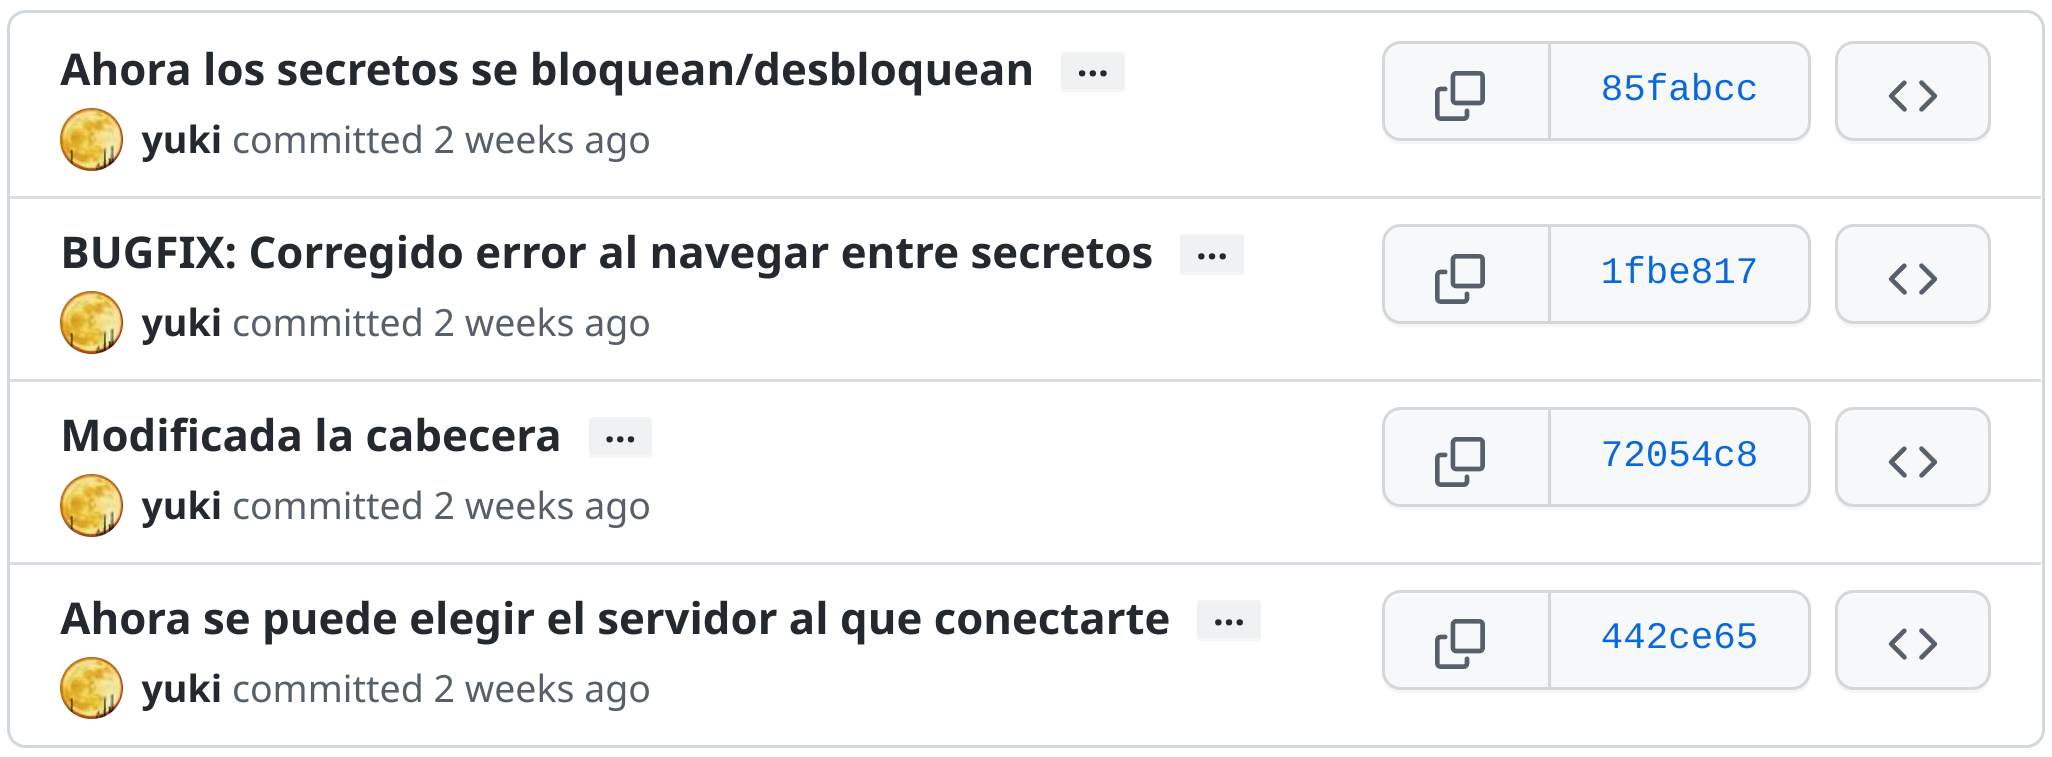
\includegraphics[width=0.8\linewidth]{img/commits.png}
%    \captionof{figure}{Histórico de varios commits realizados}
%\end{center}
%
%Aparte, también se ha integrado con Trello (a través de los plugins conocidos como “Power-Ups”) para así poder asociar las tareas a los commits que las han cumplimentado. De esta manera conseguiremos una relación “tarea ↔ código” que podremos utilizar para analizar si ha habido algún error durante el desarrollo, o fases como la de \textit{testing}.


%\subsection{Creación de entornos con Docker}
%Como dice \textcite{mouat}, los contenedores son un concepto que lleva existiendo décadas en sistemas Unix (con el comando “chroot”), pero \href{https://es.wikipedia.org/wiki/Docker_(software)}{Docker} cogió la tecnología existente de contenedores Linux y la amplió de varias maneras, sobre todo gracias a su sistema de imágenes portable.
%
%Gracias a utilizar distintas imágenes Docker con distintos servicios, se ha podido realizar despliegues de manera sencilla para distintos entornos (desarrollo, test y producción).
%
%También ha sido especialmente útil al poder realizar el desarrollo en distintos ordenadores, sin perder el tiempo en realizar instalaciones de librerías y ejecutables, creando el entorno de desarrollo en segundos.




\chapter{Metodologías utilizadas}

Hoy en día es conveniente hacer uso de las \textbf{metodologías ágiles} cuando realizamos la gestión de un proyecto, ya que cuentan con una serie de ventajas que nos van a permitir dar una respuesta más rápida y flexible ante posibles cambios durante la vida de desarrollo del producto.

Ventajas que podemos destacar de las metodologías ágiles:

\begin{itemize}
    \item Poder entregar resultados funcionales al cliente cada poco tiempo y así obtener \textit{feedback} de lo realizado.
    \item Seremos capaces de dar una respuesta ágil y flexible ante posibles cambios que puedan surgir (cambios en los requisitos, ante bajas de personal asignado al proyecto, dificultades durante el desarrollo...).
    \item Tratar de evitar burocracia innecesaria, para centrarnos de esta manera en el producto y sus funcionalidades.
    \item Tratar de involucrar al cliente (y/o a los usuarios finales) y colaborar con él, para de esta manera conseguir un mayor valor al producto.
\end{itemize}

\section{Gestión del proyecto}

Para comenzar con la gestión del proyecto debemos contar con los requisitos listados previamente y transformarlos en las conocidas como “\textbf{historias de usuario}”.

En ellas plasmaremos, en un lenguaje sencillo de entender, las funcionalidades que el producto debe tener, a las que asociaremos otros datos como son:

\begin{itemize}
    \item Un \textbf{identificador único} para poder diferenciarlas del resto.
    \item Una \textbf{estimación de tiempos} de lo que creemos que podemos tardar en realizarlo.
    \item La \textbf{prioridad} inicial para poder ordenarlas entre ellas.
    \item El \textbf{tema principal} al que se relaciona la historia de usuario.
    \item Se añadirán posibles \textbf{dependencias} de otras historias de usuario.
    \item Una \textbf{descripción} de lo que se quiere conseguir.
    \item Unos \textbf{criterios de validación} por parte del cliente.
\end{itemize}

Teniendo en cuenta los datos que queremos plasmar en las “historias de usuario”, y tras haber realizado el análisis de los requisitos del proyecto, veremos cuál ha sido el resultado obtenido en el siguiente apartado.


\subsection{Resultado del análisis realizado}

A continuación se van a identificar las distintas “historias de usuario” obtenidas, en las que se ha ido plasmando la información necesaria que posteriormente se utilizarán para la creación de las tareas a desarrollar:

\begin{requisitostbl}{X[1]X[2]X[2]X[3]X[2]}
    ID & Estimación & Prioridad  & Tema &  Dependencias \\
    1  & 25 horas & 1  & Interfaz web &   \\

    Desarrollar “esqueleto” del interfaz web \\

    \textbf{Descripción}:
    Como usuario necesito un interfaz web para poder acceder a la aplicación y hacer uso de ella. Es la base del proyecto. \\

    \textbf{Criterios de validación}:
    El interfaz es \textit{\textbf{responsive}}, visualmente atractivo y funcional. \\
\end{requisitostbl}

\begin{requisitostbl}{X[1]X[2]X[2]X[3]X[2]}
    ID & Estimación & Prioridad  & Tema &  Dependencias \\
    2  & 10 horas & 1  & Gestión de usuarios & 1  \\

    Crear “login” de usuario \\

    \textbf{Descripción}:
    Como usuario quiero poder acceder a la aplicación utilizando como sistema de autenticación un usuario y contraseña.  \\

    \textbf{Criterios de validación}:
    Los valores introducidos serán autenticados contra el \textit{backend} que se decida (base de datos o LDAP/Active Directory inicialmente). \\
\end{requisitostbl}

\begin{requisitostbl}{X[1]X[2]X[2]X[3]X[2]}
    ID & Estimación & Prioridad  & Tema &  Dependencias \\
    3  & 10 horas & 1  & Gestión de Secretos & 2  \\

    Crear secretos \\

    \textbf{Descripción}:
    Como usuario quiero poder crear un secreto para poder guardar documentación sensible y/o contraseñas. \\

    \textbf{Criterios de validación}:
    \begin{itemize}
        \item El botón para crear siempre será visible.
        \item Se podrá elegir la ruta (por defecto será donde nos encontramos) y el nombre del secreto.
    \end{itemize}
    \\
\end{requisitostbl}



\begin{requisitostbl}{X[1]X[2]X[2]X[3]X[2]}
    ID & Estimación & Prioridad  & Tema &  Dependencias \\
    4  & 30 horas & 1  & Gestión de Secretos & 2, 3  \\

    Listado de secretos \\

    \textbf{Descripción}:
    Como usuario quiero poder obtener un listado de los secretos existentes para poder navegar por ellos y seleccionar el que me interese. \\

    \textbf{Criterios de validación}:
    \begin{itemize}
        \item El listado completo se visualiza mediante un árbol jerarquizado.
        \item También se puede navegar como si fuera un explorador de archivos.
        \item El interfaz mostrará un \textit{breadcrumb} para indicar la ruta en la que nos encontramos.
        \item Se puede buscar por el nombre de los secretos.
    \end{itemize}
    \\
\end{requisitostbl}


\begin{requisitostbl}{X[1]X[2]X[2]X[3]X[2]}
    ID & Estimación & Prioridad  & Tema &  Dependencias \\
    5  & 15 horas & 2  & Gestión de Secretos & 2, 3, 4  \\

    Visualizar un secreto \\

    \textbf{Descripción}:
    Como usuario quiero acceder a un secreto para visualizar su contenido.  \\

    \textbf{Criterios de validación}:
    \begin{itemize}
        \item La visualización mostrará el secreto en formato HTML.
        \item Al acceder a un secreto “bloqueado” el sistema lo debe alertar y no se permitirá editarlo.
        \item El interfaz nos mostrará la última vez que se modificó el secreto.
        \item Al visualizar el secreto aparecerán botones con distintas acciones que se podrán realizar sobre él (editar, imprimir, ver históricos, borrar).
    \end{itemize}
    \\
\end{requisitostbl}


\begin{requisitostbl}[long]{X[1]X[2]X[2]X[3]X[2]}
    ID & Estimación & Prioridad  & Tema &  Dependencias \\
    6  & 35 horas & 2  & Gestión de Secretos & 2, 3  \\

    Modificar un secreto \\

    \textbf{Descripción}:
    Como usuario quiero poder editar un secreto para realizar modificaciones.  \\

    \textbf{Criterios de validación}:
    \begin{itemize}
        \item La modificación se realizará a través de un editor \textit{\textbf{WYSIWYG}}.
        \item El editor permitirá realizar modificaciones en formato \href{https://es.wikipedia.org/wiki/Markdown}{Markdown}.
%        \item El editor permitirá guardar el secreto y al hacerlo volveremos a la visualización del mismo.
        \item Al editar el secreto se pondrá en estado “bloqueado”.
    \end{itemize}
    \\
\end{requisitostbl}

%\vspace{20pt}

\begin{requisitostbl}{X[1]X[2]X[2]X[3]X[2]}
    ID & Estimación & Prioridad  & Tema &  Dependencias \\
    7  & 10 horas & 3  & Gestión de Secretos & 2, 3, 5  \\

    Borrado de secretos \\

    \textbf{Descripción}:
    Como usuario quiero poder borrar secretos para que desaparezcan.  \\

    \textbf{Criterios de validación}:
    \begin{itemize}
        \item Antes de borrar debe existir un mensaje de confirmación.
        \item Al borrar un secreto, el árbol de secretos se debe actualizar.
    \end{itemize}
     \\
\end{requisitostbl}

\vspace{20pt}

\begin{requisitostbl}{X[1]X[2]X[2]X[3]X[2]}
    ID & Estimación & Prioridad  & Tema &  Dependencias \\
    8  & 15 horas & 3  & Gestión de Secretos & 2  \\

    Permitir gestionar ficheros como secretos \\

    \textbf{Descripción}:
    Como usuario quiero poder subir ficheros al sistema para guardarlos cifrados.  \\

    \textbf{Criterios de validación}:
    \begin{itemize}
        \item Se permite subir cualquier tipo de fichero.
        \item Se permite descargar el fichero original.
        \item Se debe poder visualizar los ficheros más habituales en la propia web (imágenes y ficheros PDF) sin necesidad de descargarlos.
    \end{itemize}
     \\
\end{requisitostbl}

\vspace{20pt}

\begin{requisitostbl}{X[1]X[2]X[2]X[3]X[2]}
    ID & Estimación & Prioridad  & Tema &  Dependencias \\
    9  & 20 horas & 4  & Gestión de Secretos & 3, 6  \\

    Versionado de secretos\\

    \textbf{Descripción}:
    Como usuario quiero poder ver las veces que el fichero ha sido modificado para poder ver los cambios realizados.  \\

    \textbf{Criterios de validación}:
    \begin{itemize}
        \item Poder ver el número de versiones que tiene un secreto.
        \item Poder ver una versión concreta del secreto.
        \item Poder ver las diferencias entre versiones.
        \item Poder restaurar una versión concreta del secreto.
    \end{itemize} \\
\end{requisitostbl}


\begin{requisitostbl}{X[1]X[2]X[2]X[3]X[2]}
    ID & Estimación & Prioridad  & Tema &  Dependencias \\
    10  & 5 horas & 4  & Gestión de Secretos & 2, 5  \\

    Imprimir secretos \\

    \textbf{Descripción}:
    Como usuario quiero poder imprimir un secreto. \\

    \textbf{Criterios de validación}:
    Existe un botón para imprimir un secreto. \\
\end{requisitostbl}

\vspace{10pt}

\begin{requisitostbl}{X[1]X[2]X[2]X[3]X[2]}
    ID & Estimación & Prioridad  & Tema &  Dependencias \\
    11  & 35 horas & 2  & Producción & 1  \\

    Puesta en producción segura \\

    \textbf{Descripción}:
    Como usuario quiero poder acceder a la plataforma de manera segura para realizar todo lo comentado hasta ahora \\

    \textbf{Criterios de validación}:
    \begin{itemize}
        \item El acceso web tiene que ser por HTTPS (certificado válido).
        \item El servidor debe estar securizado ante accesos externos.
        \item Los servicios deben auto-arrancarse en caso de caída.
        \item Existe un registro de lo sucedido a cada secreto (auditoría).
    \end{itemize} \\
\end{requisitostbl}
\vspace{10pt}

\subsection{Mapa de las historias de usuario}

Dado que las historias de usuario pueden suponer la agrupación de distintas tareas técnicas que son más pequeñas, es conveniente crear un mapa que englobe todas las tareas a realizar.

Para la organización de este mapa se pueden identificar los siguientes apartados:
\begin{itemize}
    \item Los \textbf{temas} son las características a alto nivel que va a tener la aplicación, y coinciden con el tema de las historias de usuario. En el mapa se ha diferenciado en color verde.
    \item Los \textbf{epics}, en color azul, son características que normalmente no pueden realizarse en un \textit{sprint}, que a veces pueden ser divididas en distintas historias de usuarios, y que engloban en su mayoría varias tareas.
    \item Las \textbf{tareas}, en este caso en amarillo, son las unidades concretas de trabajo. Se ha tratado que sean lo más cortas posibles y que a nivel técnico sean auto-contenidas y aisladas.
\end{itemize}

El mapa resultante inicial para la gestión del proyecto es el siguiente:

\begin{center}
    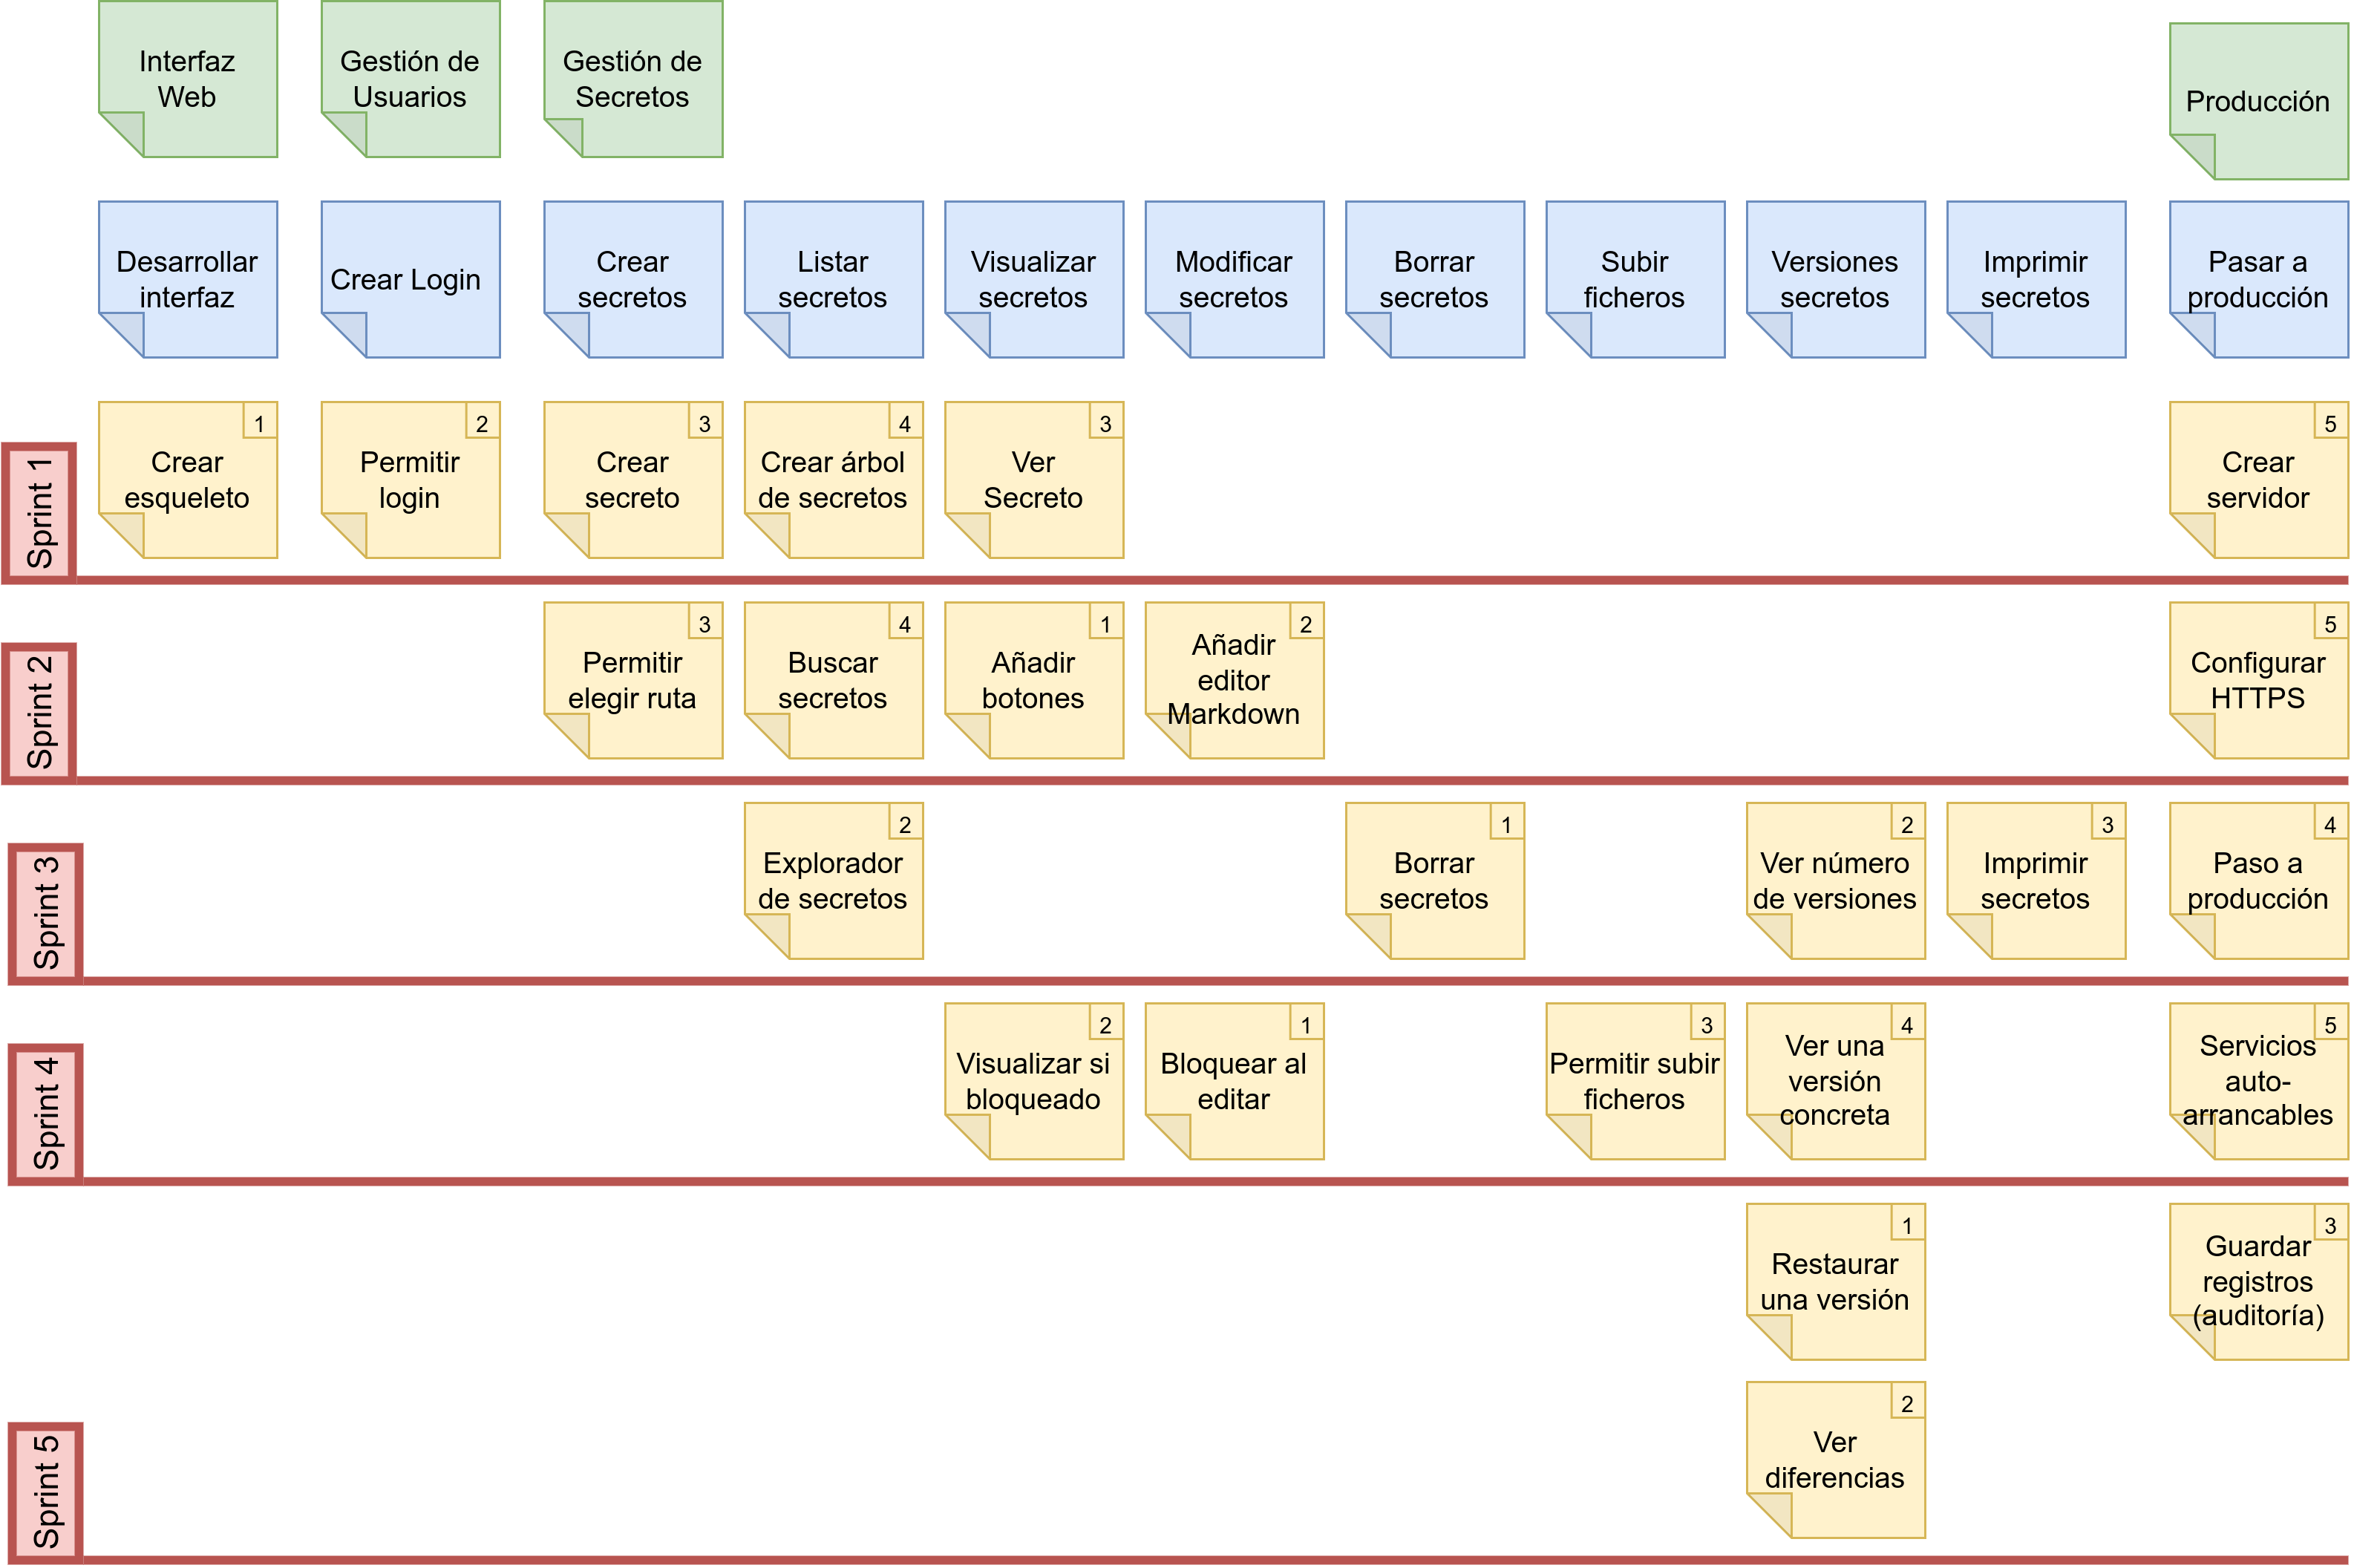
\includegraphics[width=\linewidth]{img/kanban.png}
    \captionof{figure}{Mapa de las tareas a realizar}
\end{center}

\subsection{\textit{Sprints} generados}

A la par que se ha ido creando el mapa anterior, se han diferenciado diferentes \textit{sprints} con las tareas que deberían completarse para cada uno de ellos.

Bien es cierto que aunque haya sido realizada esa primera estimación, se podrían efectuar modificaciones en caso de que fuese necesario.

Para el primer \textit{sprint} se han identificado las siguientes tareas que deben realizarse:

\begin{center}
    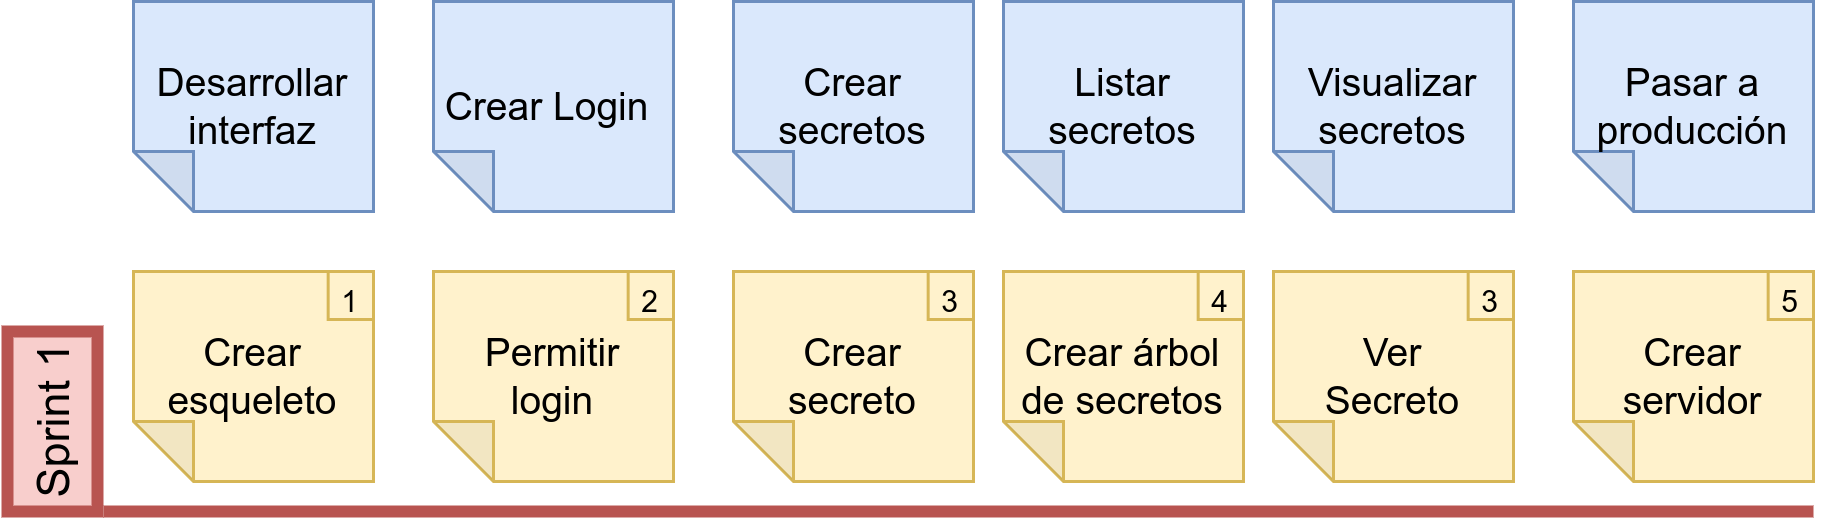
\includegraphics[width=\linewidth]{img/sprint1.png}
    \captionof{figure}{Tareas a realizar en el \textit{Sprint} 1}
\end{center}

Tal como se puede ver, las tareas están representadas con su prioridad dentro del \textit{sprint}, para así también tener claro qué tareas deben tratar de terminarse antes que otras.

Al terminar este primer \textit{sprint}, tendremos la base del proyecto terminada, y podríamos mostrarle al cliente una primera versión con unas funcionalidades básicas.

De esta manera, podemos obtener \textit{feedback} de lo realizado, con una base ya terminada. Ese \textit{feedback} podremos utilizarlo como retroalimentación para el siguiente \textit{sprint}, ya sea para realizar modificaciones de lo ya realizado (hacer cambios nuevos que el cliente pida) o para utilizarlo para las tareas ya planificadas.

Para llevar una mejor gestión de las tareas expuestas en este apartado, lo ideal es utilizar un software especializado creado con dicho objetivo, como el que vamos a analizar a continuación.

\section{Gestión de tareas con Trello}

\href{https://trello.com/}{Trello} es una aplicación web, creada por la empresa \href{https://www.atlassian.com/}{Atlassian}, que nos permite tener un tablero \href{https://en.wikipedia.org/wiki/Kanban_(development)}{Kanban} donde podremos añadir las tareas de nuestro proyecto, e ir moviéndolas entre distintas etapas.

Aunque cuenta con una versión de suscripción, la versión gratuita dispone de las características suficientes como para poder ser utilizado para la gestión de proyectos sin ningún problema.

Una vez definidas las tareas, tal como se ha visto anteriormente, se han añadido a Trello, en el que se han creado diferentes columnas, o fases de desarrollo.

Aparte, y para que a nivel visual sea más sencillo de determinar de qué tipo es cada tarea, a cada una de ellas se les ha asignado un color teniendo en cuenta el tema al que pertenecen, y varias etiquetas que representan el \textit{sprint} y la prioridad dentro del \textit{sprint}. De esta manera, Trello nos permitirá realizar búsquedas o visualizar las tareas con la etiqueta que nos interese.


\begin{center}
    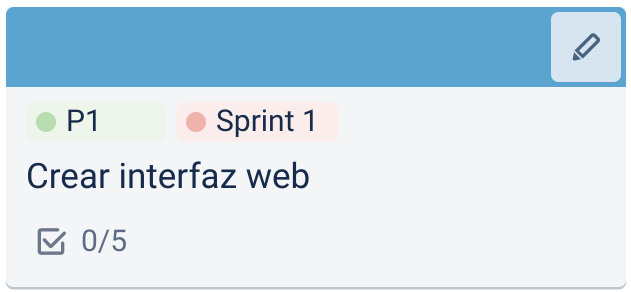
\includegraphics[width=0.5\linewidth]{img/tarea.png}
    \captionof{figure}{Detalle de la tarea}
\end{center}

Las tareas serán movidas entre las diferentes fases de desarrollo a medida que se van realizando. Se ha determinado contar con las siguientes fases:


\begin{minipage}{0.60\linewidth}
    \begin{itemize}
        \item \textbf{Tareas pendientes}: donde situaremos las tareas que se deben realizar para llevar a cabo el proyecto.
        \item \textbf{Desarrollo}: Son las tareas que se han empezado a desarrollar.
        \item \textbf{Testing}: Son las tareas que se dan por terminadas en el desarrollo y que pasan a una fase de testeo. En algunos casos puede ser directamente testeado por el cliente para dar su feedback (por ejemplo para el interfaz web), aunque lo habitual es que el testeo lo realice otra persona del proyecto (que no haya sido quien ha hecho el desarrollo).

        En caso de que una tarea no pase esta fase, se anotará los inconvenientes y volverá a la columna de \textbf{desarrollo}.
        \item \textbf{Producción}: Una vez el \textit{testing} ha terminado, se puede dar por terminada la tarea y podrá ser incluida en producción.
    \end{itemize}

    Tal como se puede ver en la imagen, cada tarea se representa como una pequeña tarjeta, apareciendo como un listado de todas ellas en la columna correspondiente en las que están situadas (en este caso todavía en la lista de tareas pendientes).
\end{minipage}
\hfill
\begin{minipage}{0.32\linewidth}
    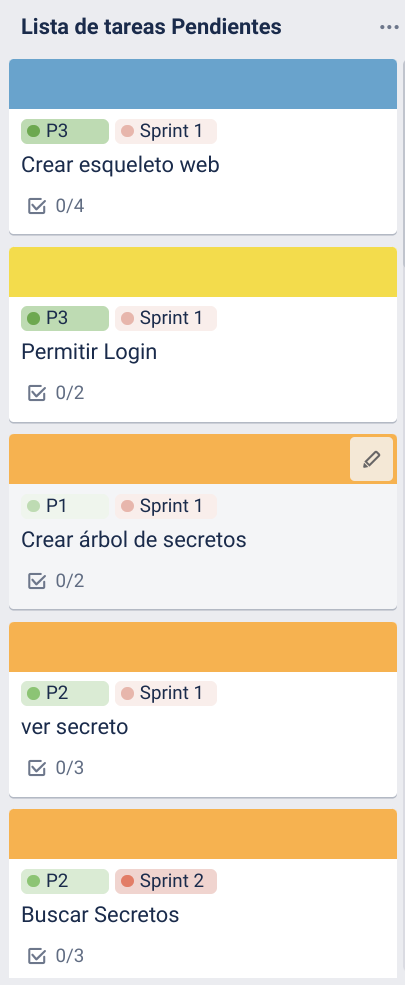
\includegraphics[width=\linewidth]{img/tareas.png}
    \captionof{figure}{Tareas pendientes en Trello}
\end{minipage}

%\vspace{10pt}



%\hfill


Por último, cada tarea puede tener un listado de pequeños ítems. Estos han sido detallados para que a la hora de desarrollar se tenga en cuenta qué es lo que se debe conseguir, y de esta manera dar por finalizada la tarea.
\begin{center}
    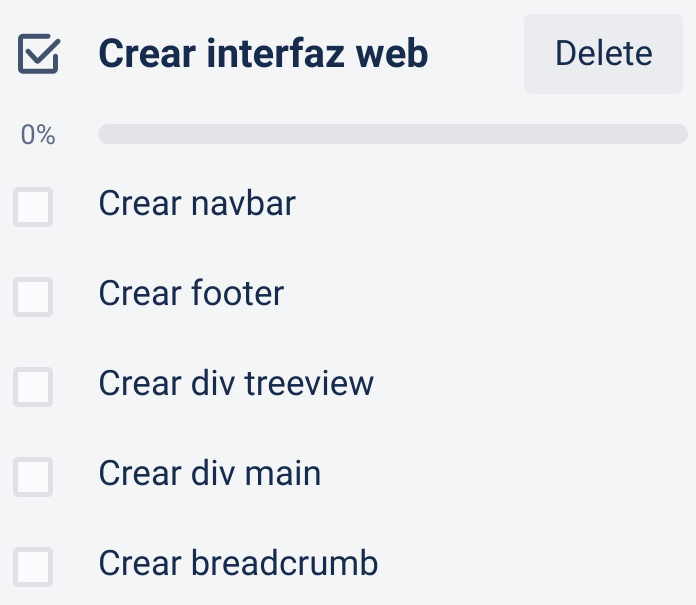
\includegraphics[width=0.4\linewidth]{img/tarea1.png}
    \captionof{figure}{Ítems de la tarea}
\end{center}

Tras terminar la tarea, se pasará a la columna \textbf{testing}, para de esta manera, tal como se ha dicho previamente, comenzar con la fase de testeo.



\chapter{Resultados obtenidos}

A continuación se va a exponer los pasos realizados para el diseño y la creación de la aplicación teniendo en cuenta los requisitos del proyecto y las historias de usuario detalladas previamente. Se van a diferenciar distintos apartados generales:
\vspace{-10pt}
\begin{itemize}
    \item Diseño del \textbf{interfaz}
    \item \textbf{Angular}: Aspectos destacables de la programación
    \item \textbf{Características y uso} de la aplicación
\end{itemize}


\section{Diseño del interfaz}

El interfaz web de la aplicación es el punto de entrada del usuario, por lo que es importante dedicarle el esfuerzo que se merece ya que puede determinar el éxito o el fracaso en el uso de la aplicación.

A la hora de hacer el diseño, se han tenido en cuenta:
\vspace{-10pt}
\begin{itemize}
    \item \textbf{Facilidad de uso}: Es importante que la aplicación tenga una buena usabilidad, para que el usuario final no requiera de ningún esfuerzo a la hora de utilizarla.
    \item \textbf{Diseño funcional}: Continuando con el punto anterior, se ha tratado de realizar un diseño funcional, para que cada parte de la interfaz se sepa para qué va a ser utilizada. Para facilitarlo, se ha trabajado tratando de conseguir un diseño \textbf{minimalista}.
    \item Se ha realizado un \textbf{diseño adaptable a la pantalla} (también conocido como diseño \textit{responsive}) para facilitar el uso de la aplicación en dispositivos móviles.
\end{itemize}


\subsection{Primer boceto}
Para la creación del interfaz se decidió crear un primer prototipo a boli en un cuaderno, tratando de plasmar las ideas generales, y la colocación inicial de los elementos con los que los usuarios van a interactuar.

Este primer boceto sirve para asentar las historias de usuario y las distintas acciones que los usuarios van a poder realizar en la aplicación final. Es una manera rápida para empezar a tomar consciencia del proyecto y cómo queremos encauzar el interfaz.

\vspace{-20pt}
\begin{center}
    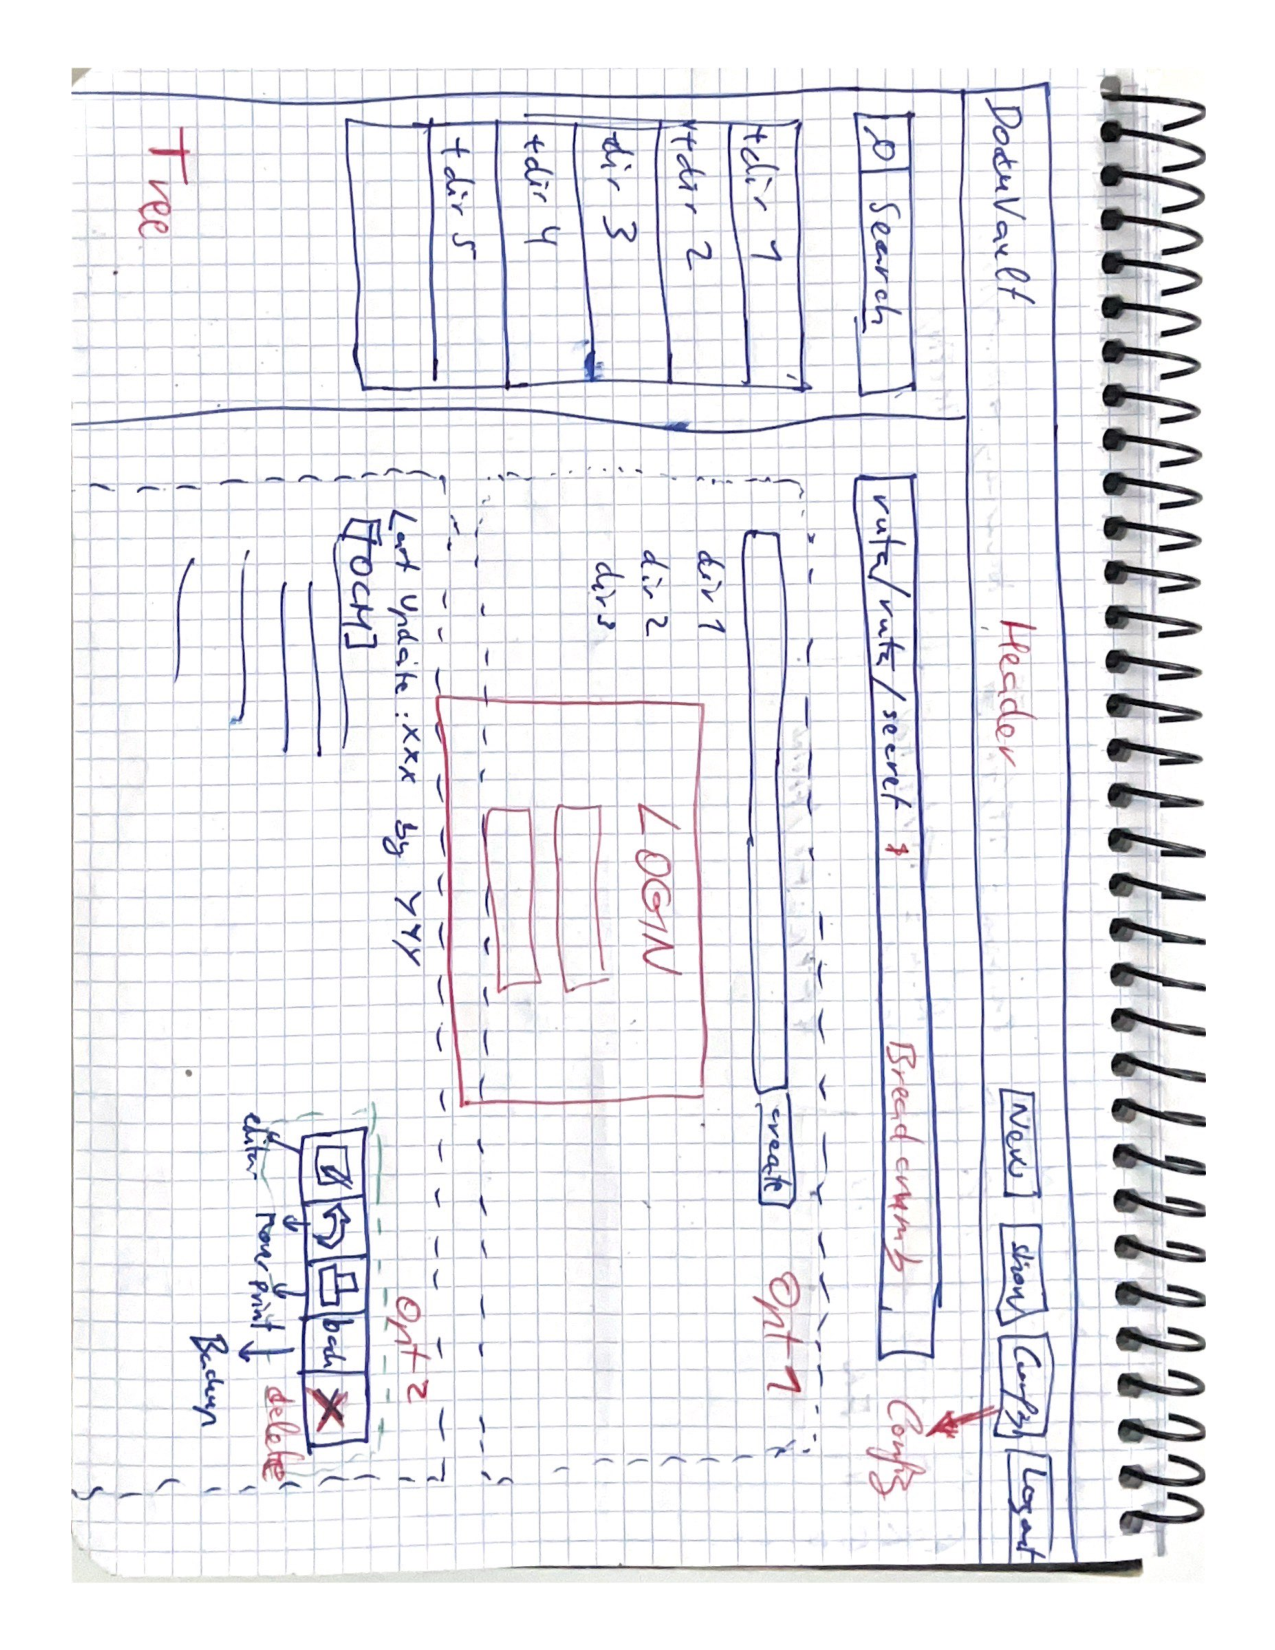
\includegraphics[angle=90,width=\linewidth]{img/boceto.pdf}
    \vspace{-20pt}
    \captionof{figure}{Boceto del interfaz}
\end{center}

En el boceto existen zonas diferenciadas hechas en color azul, donde también aparece en color rojo el nombre para cada zona. Ya en este primer boceto se estaban identificando lo que posteriormente serán distintos componentes independientes.

En rojo, en la parte central también aparece cómo sería el login, que daría paso al interfaz general. Por último, se pueden diferenciar, también en la parte central, nombrados como “Opt1” y “Opt2”, las vistas que dependerán de qué estemos haciendo: si navegamos por los secretos o si estamos visualizando/editano un secreto.

Tal como se puede ver, ya en este primer boceto se tenía una idea bastante clara de cómo debía ser a grandes rasgos el interfaz final.

\subsection{Creación inicial del interfaz con un \textit{framework} CSS}
Una vez se tuvieron claro los aspectos generales del boceto, se realizó un primer prototipo haciendo uso de un \textit{framework CSS}.

El \textit{framework} elegido ha sido \href{https://getbootstrap.com/}{Bootstrap}, ya que va a permitir crear un diseño funcional, de manera sencilla, y dispone de distintas características que  van a resultar útiles durante el uso de la aplicación (como por ejemplo los “\textit{modal}” y el “\textit{breadcrumb}”).

\begin{center}
    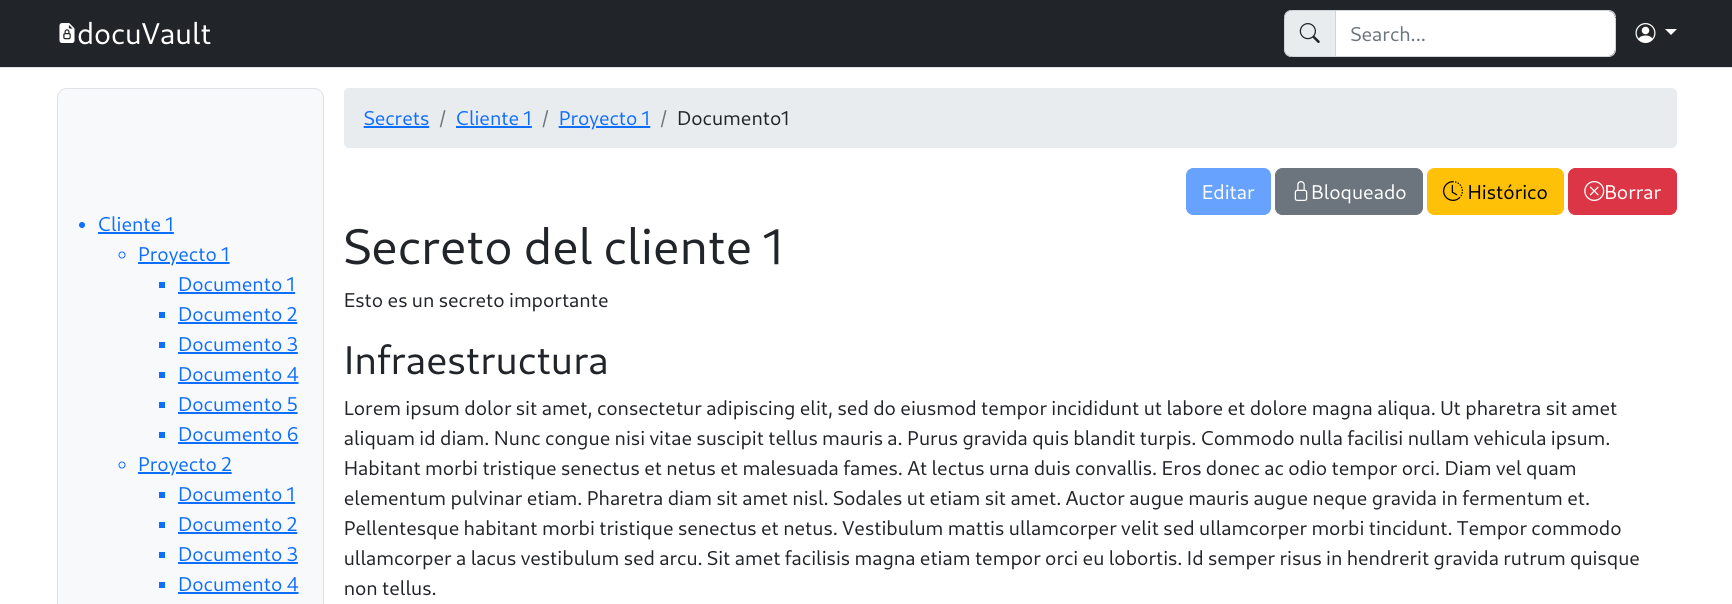
\includegraphics[frame,width=\linewidth]{img/boceto2.png}
    \vspace{-20pt}
    \captionof{figure}{Boceto del interfaz con Bootstrap y datos estáticos}
\end{center}

Bootstrap ha permitido crear un código sencillo, pero visualmente atractivo, y que posteriormente será reutilizado para el interfaz final.


\subsection{Del prototipo al código real}

Tal como se ha comentado previamente, Bootstrap permitió crear crear el prototipo del interfaz de manera rápida y sencilla. Aunque el aspecto visual a grandes rasgos no ha variado en exceso, a medida que se iba avanzando en el proyecto se han ido realizando pequeñas modificaciones.

El interfaz final se puede descomponer en distintos apartados que cumplen con distintas funcionalidades. La pantalla de \textit{\textbf{login}} nos permite introducir el usuario y la contraseña del mismo para acceder a la aplicación.


\begin{center}
    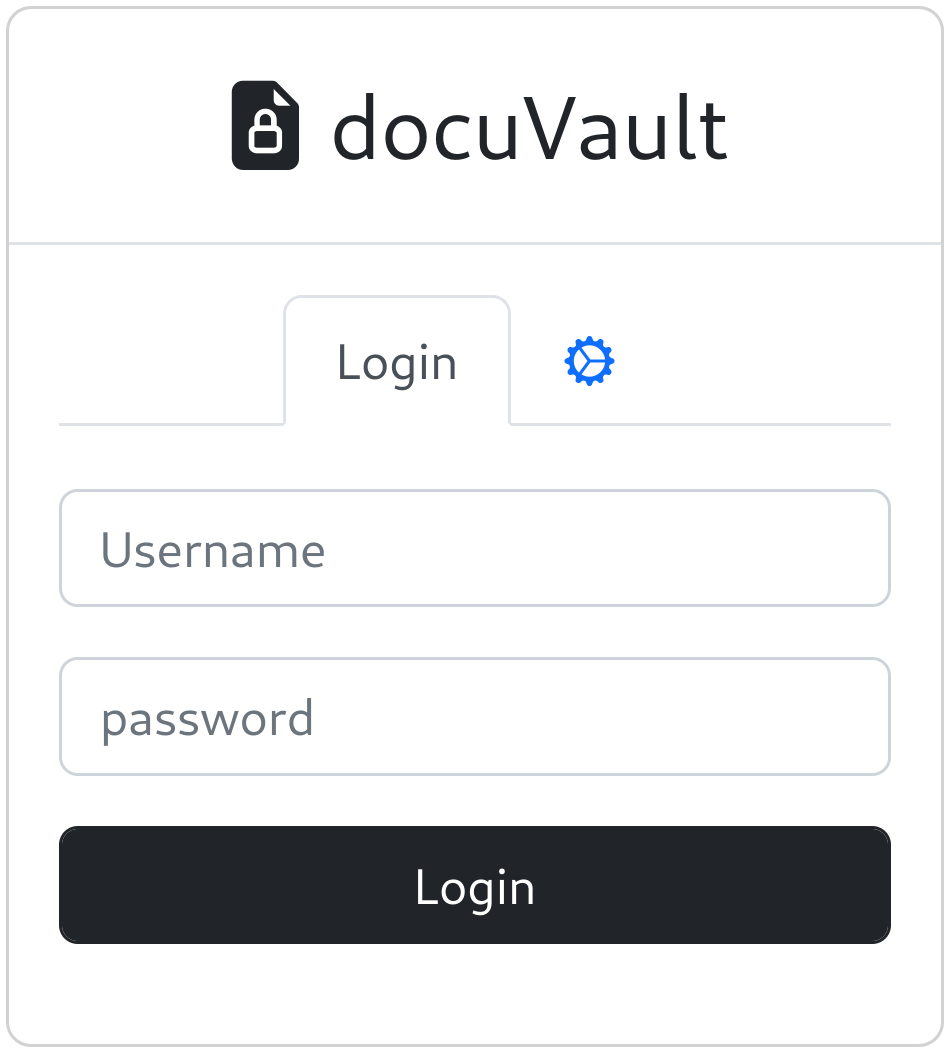
\includegraphics[width=0.4\linewidth]{img/login.png}
    \hfil
    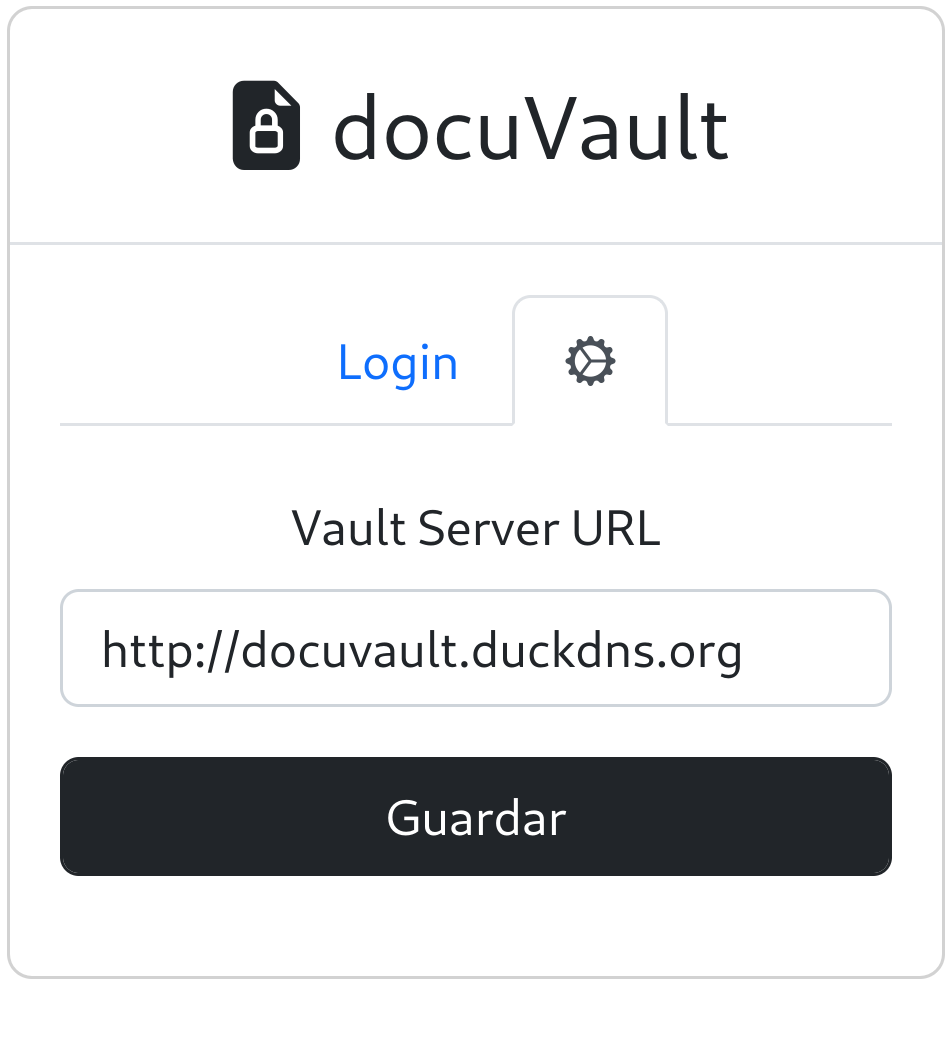
\includegraphics[width=0.4\linewidth]{img/login2.png}
%    \vspace{-10pt}
    \captionof{figure}{Interfaz para el \textit{login}}
\end{center}

En esta ventana de \textit{login} se ha añadido una pestaña extra con el símbolo del engranaje que permite modificar la URL de conexión al que nos queremos conectar

Tras realizar la autenticación la aplicación nos llevará al directorio principal donde podremos navegar a través del interfaz para acceder a los secretos que nos interese.

\begin{center}
    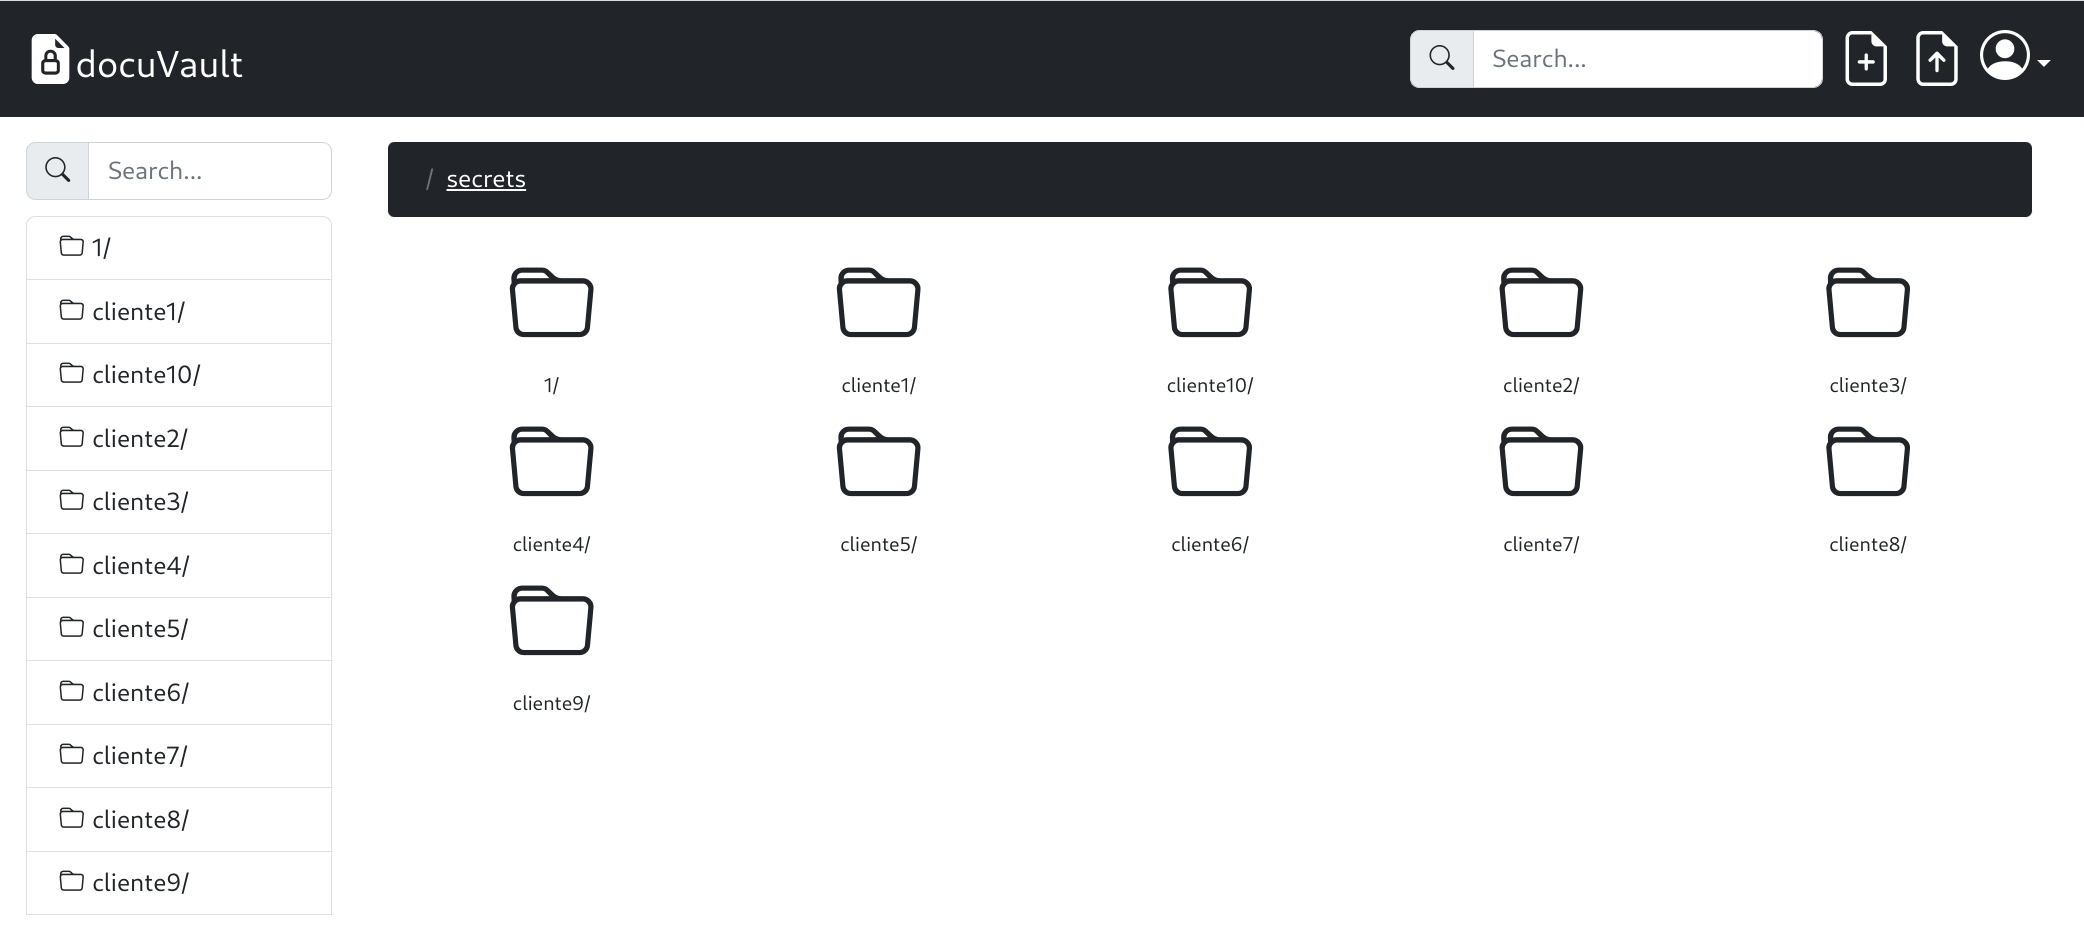
\includegraphics[frame,width=\linewidth]{img/interfaz1.png}
    %    \vspace{-10pt}
    \captionof{figure}{Interfaz principal de la aplicación}
\end{center}

Al acceder al secreto que nos interesa, el interfaz nos muestra el documento descifrado junto con unos botones con los que realizar ciertas acciones sobre los secretos.

\begin{center}
    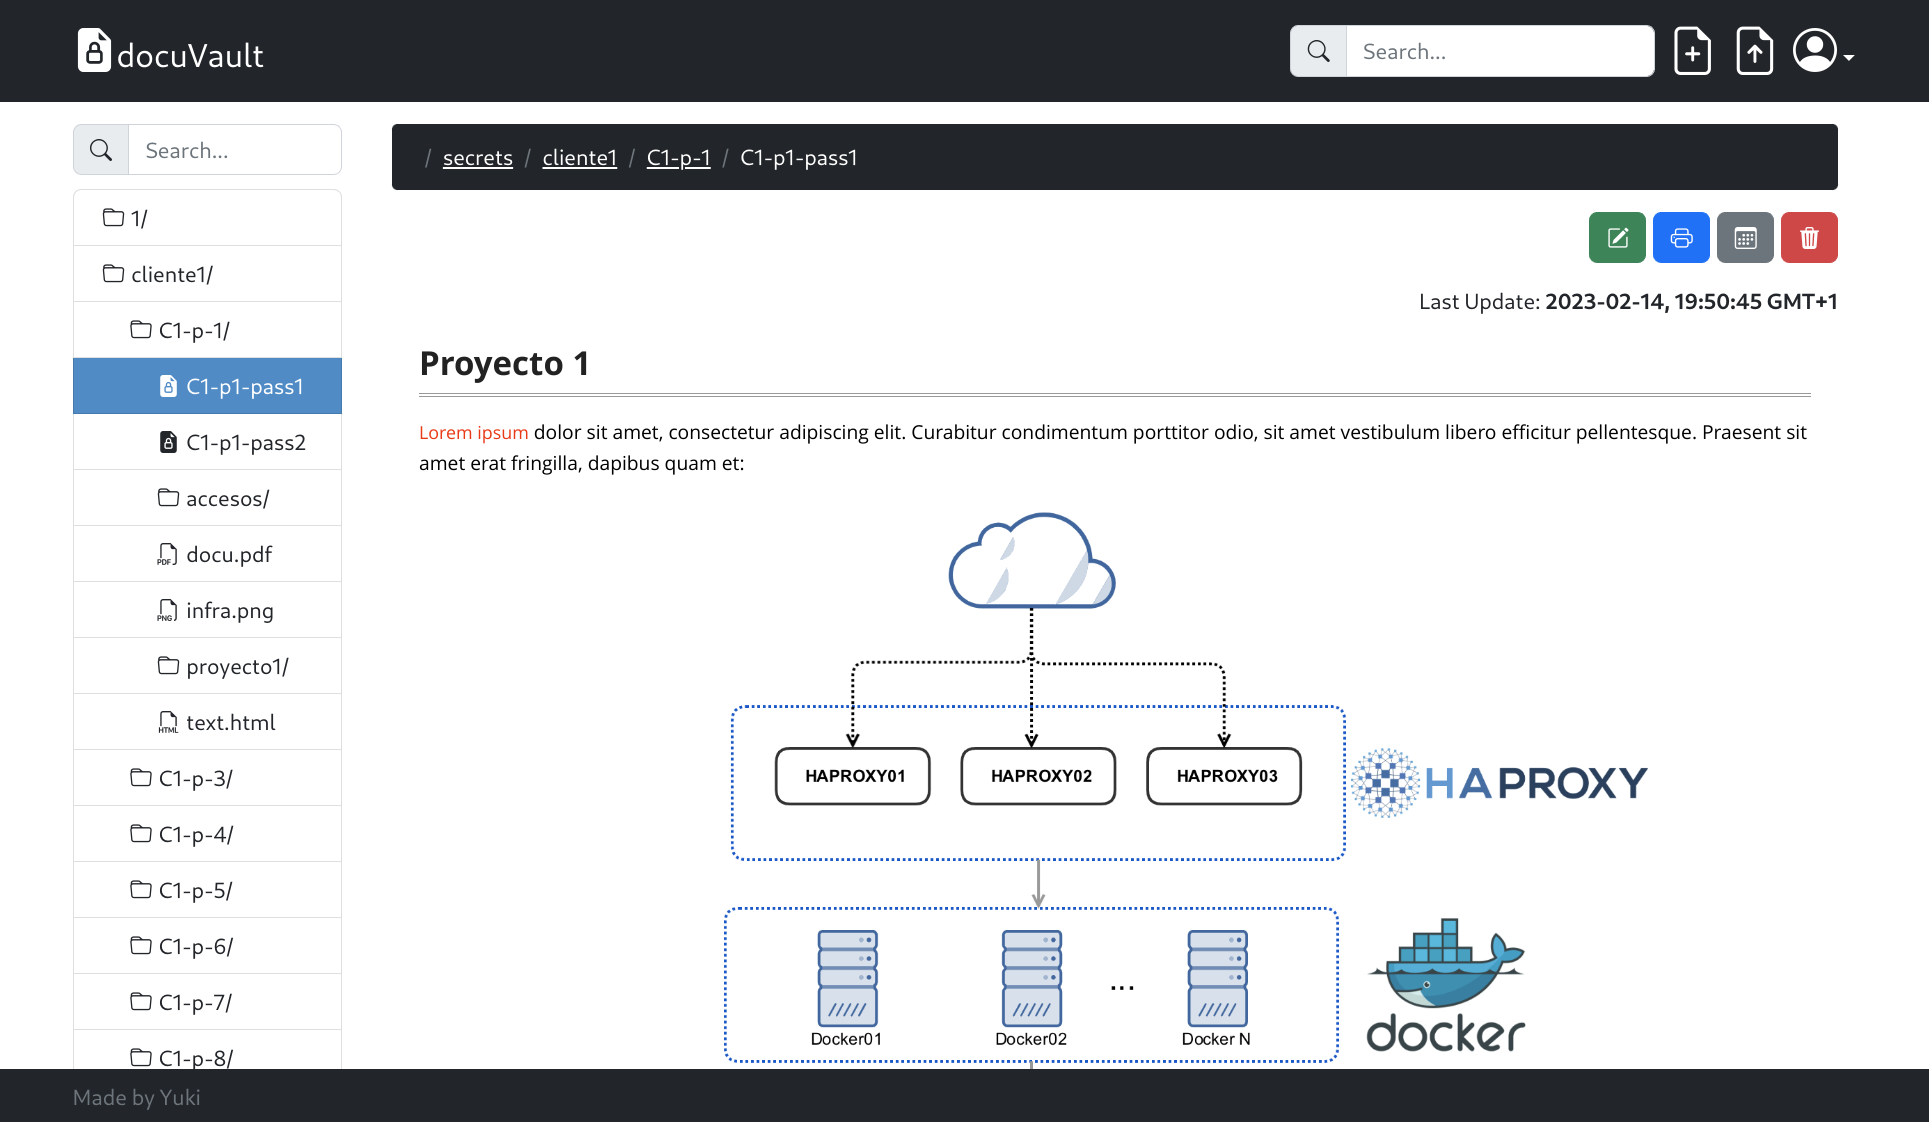
\includegraphics[frame,width=\linewidth]{img/interfaz2.png}
    %    \vspace{-10pt}
    \captionof{figure}{Interfaz al visualizar un secreto}
\end{center}



\subsection{Interfaz \textit{responsive}}

Para facilitar el uso de la aplicación en distintos tipos de pantallas, se ha hecho que el interfaz se adapte al tamaño donde se está visualizando la aplicación. Esto va a permitir que el usuario pueda acceder a través de su teléfono móvil, lo que puede ser útil en entornos de empresa donde se tengan que realizar salidas a clientes.

\begin{center}
    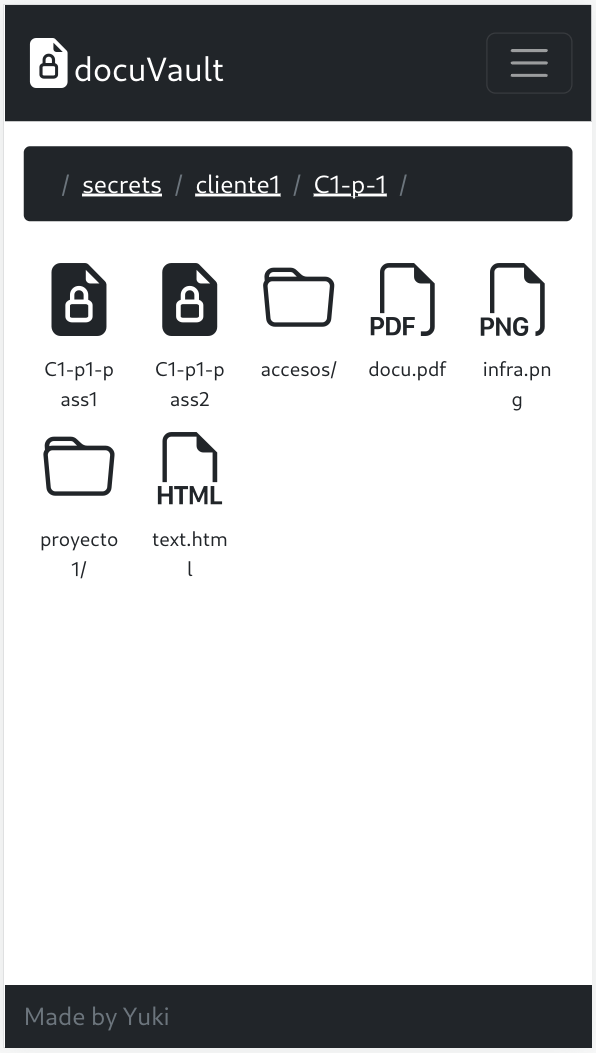
\includegraphics[width=0.3\linewidth]{img/responsive1.png}
    \hfill
    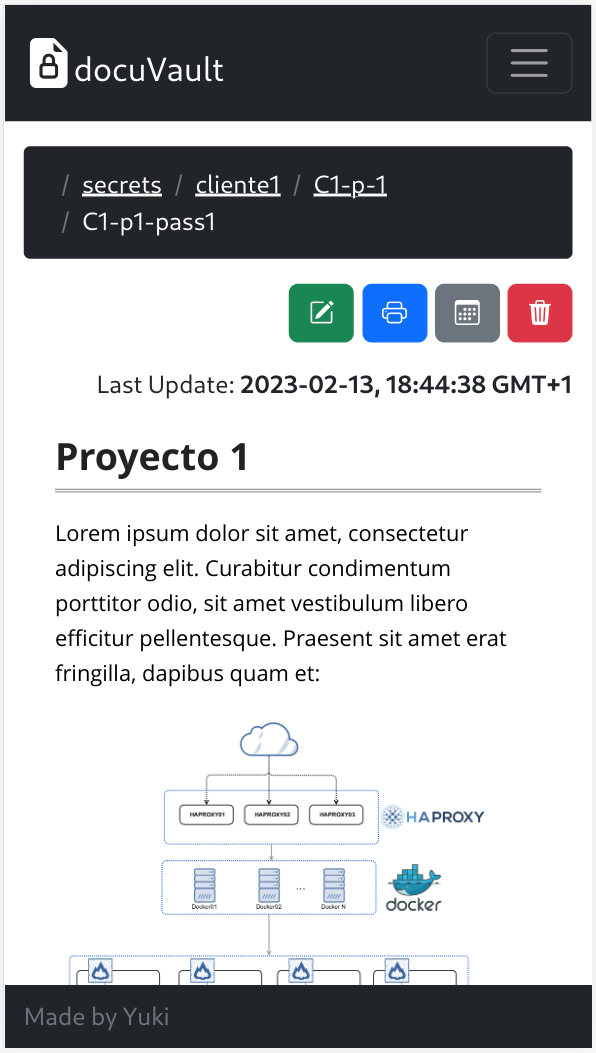
\includegraphics[width=0.3\linewidth]{img/responsive2.png}
    \hfill
    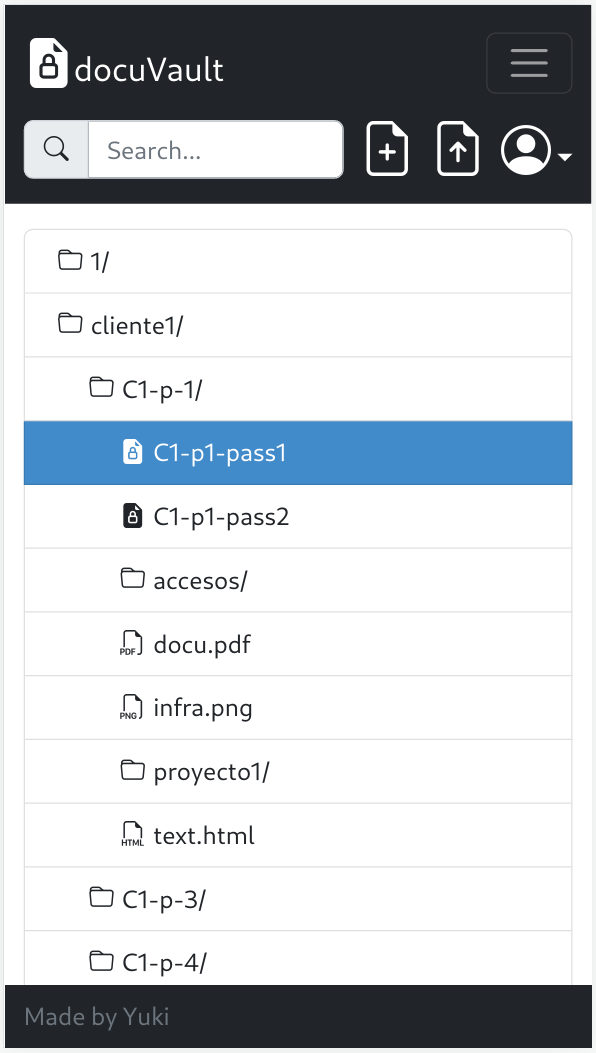
\includegraphics[width=0.3\linewidth]{img/responsive3.png}

    \captionof{figure}{Interfaz en modo \textit{responsive}}
\end{center}

Tal como se puede ver, para mejorar la navegación, el interfaz que muestra en modo árbol la jerarquía de secretos se oculta, de esta manera navegamos a través de los secretos como un explorador de archivos.


\section{Características y uso de la aplicación}

Teniendo en cuenta los requisitos planteados al inicio del proyecto, y teniendo en cuenta que la aplicación debe ser fácil de utilizar, se ha hecho que las distintas características que dispone la aplicación y el uso de la misma recuerde a aplicaciones que los usuarios ya hayan utilizado.

A continuación se van a detallar distintas características de la aplicación y cómo se crearon pensando en el usuario final.


\subsection{Creación de un secreto nuevo}

La creación de secretos es la característica principal de la aplicación, ya que con ello se va a conseguir guardar la información sensible que nos interese.


{
\begin{minipage}{0.1\linewidth}
    
\includegraphics[width=\linewidth]{img/new.png}
\end{minipage}
\hspace{0.5cm}
\begin{minipage}{0.9\linewidth}
    En la cabecera de la aplicación existe un icono que nos va a permitir crear un nuevo secreto en el sistema.

    Al hacer \textit{click} sobre el icono, nos aparecerá un \textit{modal} (una pequeña ventana emergente en el interfaz) para preguntarnos por la ruta donde queremos crear el secreto.
\end{minipage}
}

Al aparecer el \textit{modal} nos aparecerá por defecto la ruta en la que nos encontrábamos en ese instante.

\begin{center}
    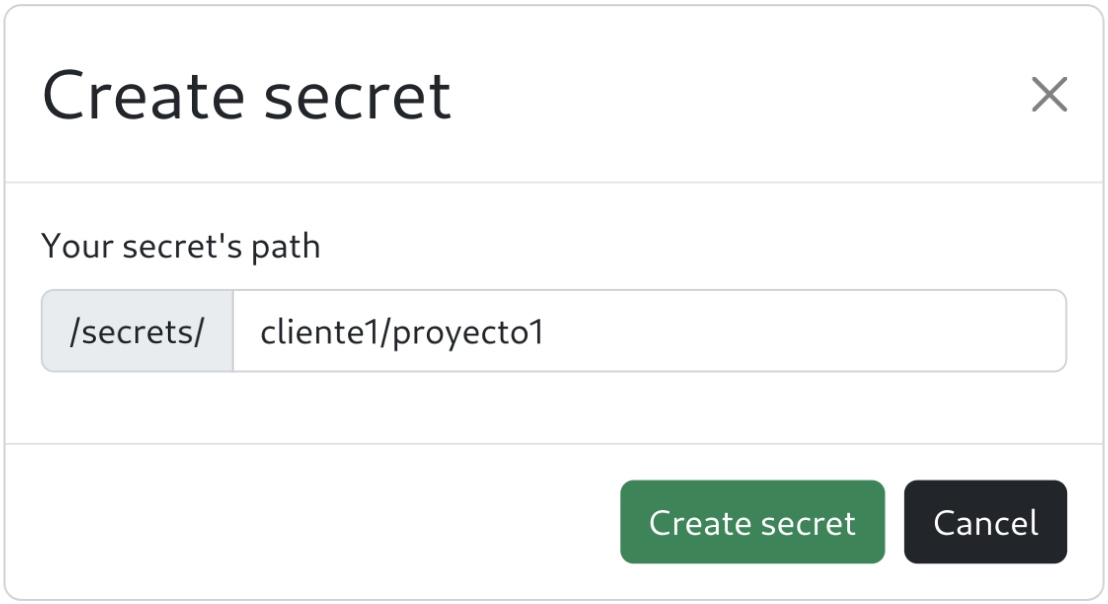
\includegraphics[width=0.7\linewidth]{img/new_secret.png}
    \captionof{figure}{\textit{Modal} para crear un secreto}
\end{center}

Si en la ruta que ponemos termina en “/” el botón para crear el secreto permanecerá deshabilitado, ya que una “barra” al final del nombre identifica un directorio, al igual que sucede en sistemas UNIX.

Al hacer \textit{click} en el botón de creación del secreto la aplicación nos creará un secreto nuevo en la aplicación y nos llevará a la ruta donde lo hemos creado.

\subsection{Acciones sobre secretos}

Una vez creado el secreto, o una vez que navegamos a un secreto creado previamente, podremos realizar distintas acciones sobre el mismo. Estas acciones dependerán de los permisos que se tengan sobre el secreto, pero a continuación se van a detallar todos ellos.

Las acciones que podremos realizar se identifican a través de  distintos iconos que nos aparecen en el interfaz y que se van a detallar a continuación.


\subsubsection*{Editar secreto}
{
\begin{minipage}{0.1\linewidth}
    
\includegraphics[width=\linewidth]{img/edit.png}
\end{minipage}
\hspace{0.5cm}
\begin{minipage}{0.9\linewidth}
    Una de las acciones principales es la de \textbf{editar el secreto}, ya sea para añadir, modificar o borrar información en el mismo. Como se verá más adelante, esta edición se hará a través de un editor completo \textit{WYSIWYG}.
\end{minipage}
}

\subsubsection*{Mover secreto}
{
\begin{minipage}{0.1\linewidth}
    
\includegraphics[width=\linewidth]{img/move.png}
\end{minipage}
\hspace{0.5cm}
\begin{minipage}{0.9\linewidth}
    Una vez creado un secreto, para realizar una reestructuración de los secretos, puede interesar moverlo. Al hacer \textit{click} en este botón se abrirá un \textit{modal} en el que nos aparecerá la ruta actual y podremos moverlo a una nueva ruta.
\end{minipage}
}
\vspace{-8pt}
\begin{center}
    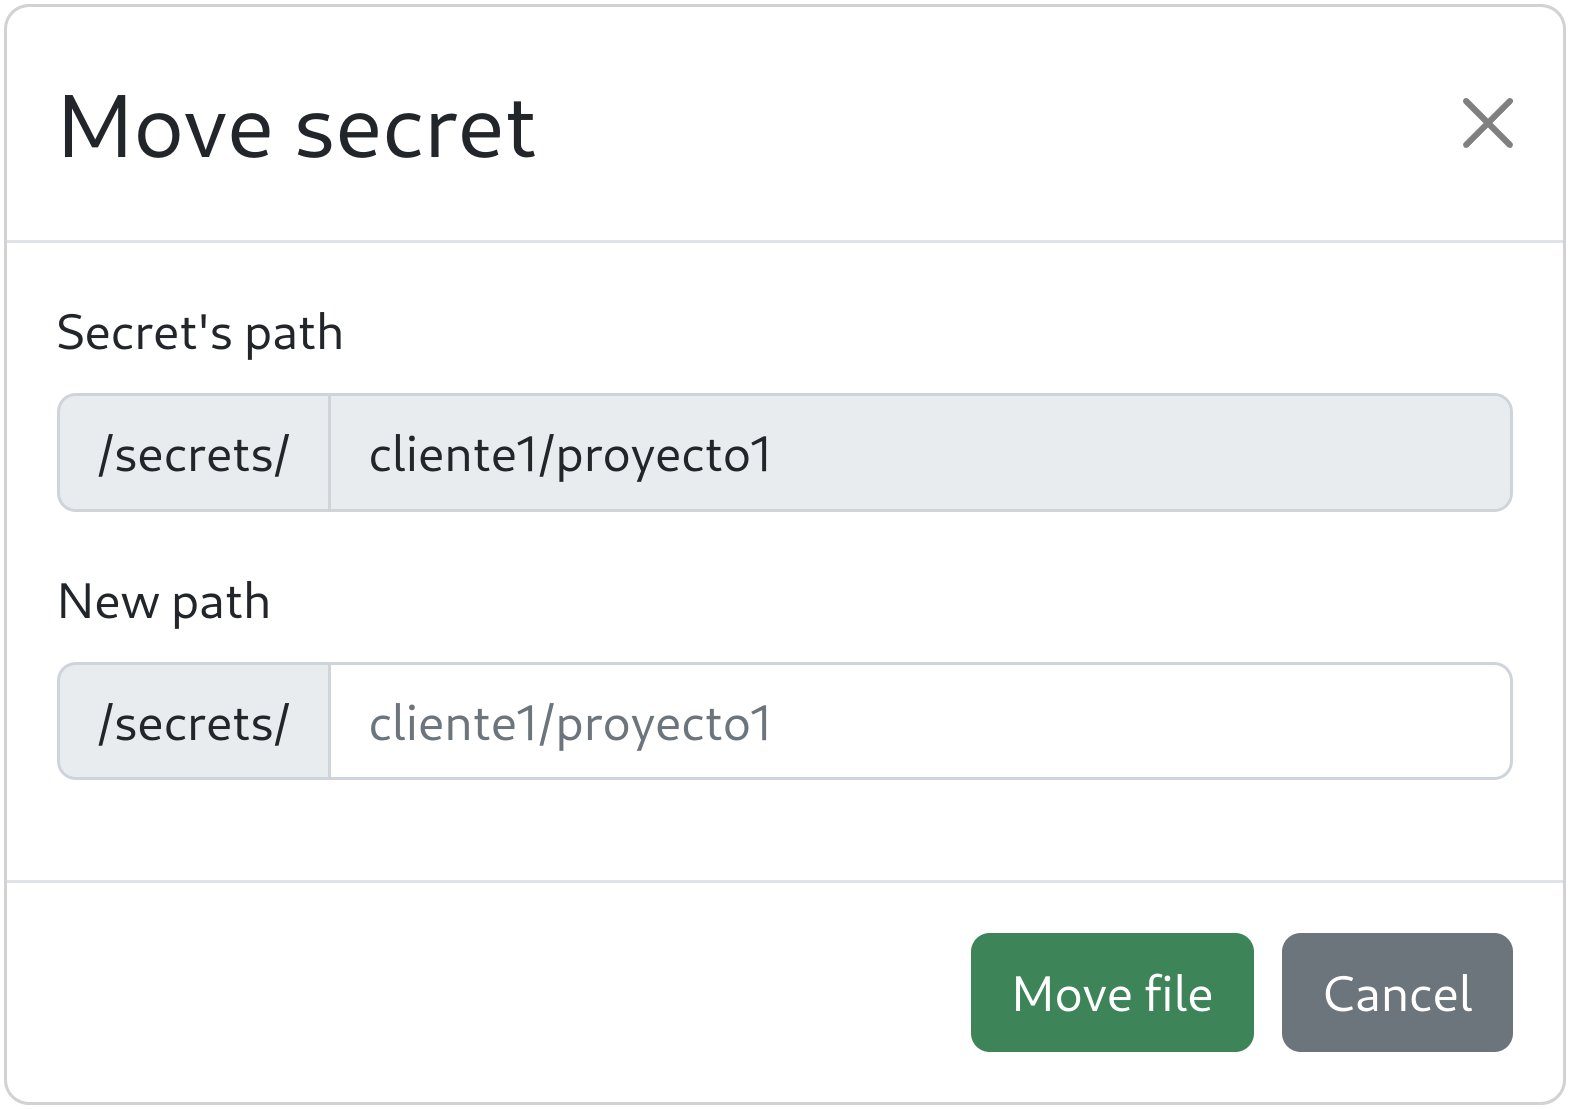
\includegraphics[width=0.56\linewidth]{img/move-modal.png}
    \captionof{figure}{Elegir nueva ruta para un secreto.}
\end{center}

\subsubsection*{Imprimir secreto}
{
\begin{minipage}{0.1\linewidth}
    
\includegraphics[width=\linewidth]{img/print.png}
\end{minipage}
\hspace{0.5cm}
\begin{minipage}{0.9\linewidth}
    En algunas ocasiones puede ser interesante \textbf{imprimir la documentación guardada}. Este icono abrirá el asistente para imprimir del navegador y nos mostrará una previsualización, en la que desaparecen partes del interfaz (la vista en árbol y los botones de acción) para mejorar el formato.
\end{minipage}
}


\subsubsection*{Visualizar histórico del secreto}
{
\begin{minipage}{0.1\linewidth}
    
\includegraphics[width=\linewidth]{img/calendar.png}
\end{minipage}
\hspace{0.5cm}
\begin{minipage}{0.9\linewidth}
    Como más adelante se explicará, cuando un secreto es modificado \textbf{se guarda un histórico} del mismo. A través de este botón podremos ver las distintas versiones del mismo e ir a una versión anterior.
\end{minipage}
}
\vspace{-8pt}
\begin{center}
    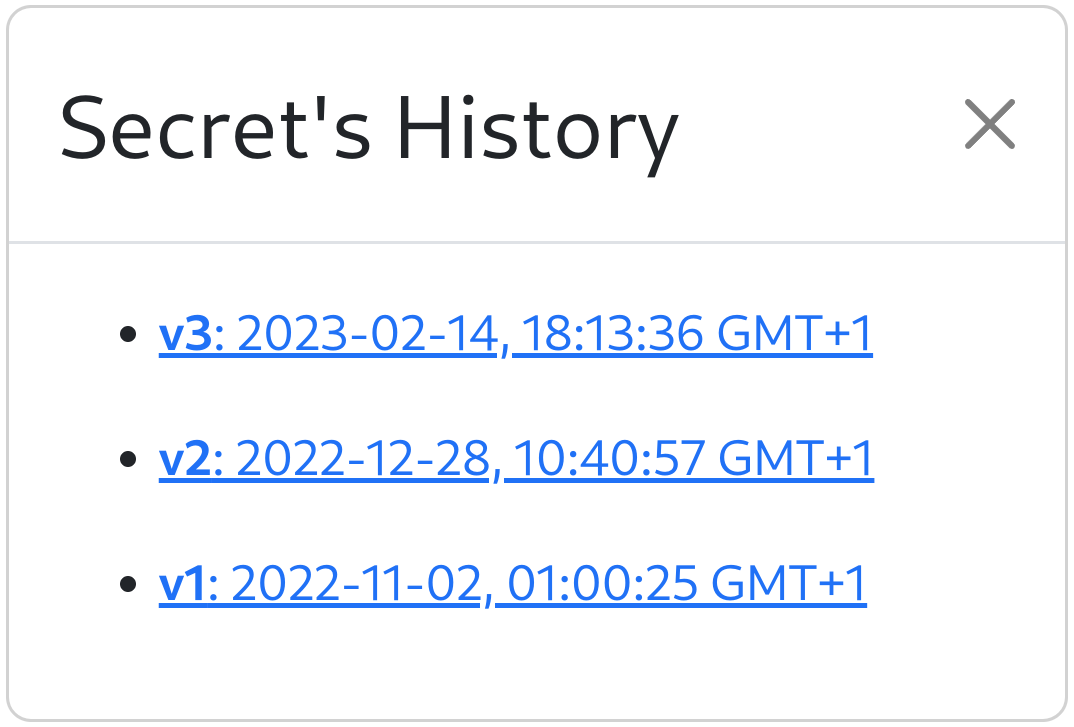
\includegraphics[width=0.56\linewidth]{img/history.png}
    \captionof{figure}{Histórico de un secreto.}
\end{center}

De esta manera, podremos ver cualquier cambio que haya sufrido el secreto a lo largo del tiempo. Al hacer \textit{click} en alguno de los enlaces para visualizar alguna versión anterior, nos aparecerá un mensaje encima del secreto para indicarlo:
\vspace{-8pt}
\begin{center}
    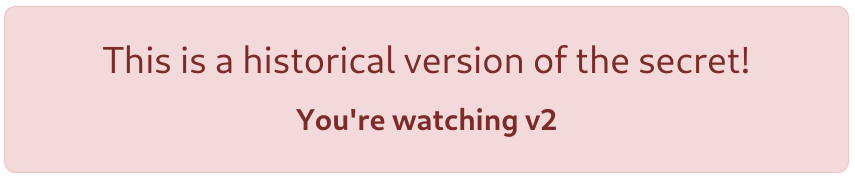
\includegraphics[width=0.6\linewidth]{img/history2.png}
    \captionof{figure}{Mensaje indicando la versión del secreto.}
\end{center}

\subsubsection*{Desbloquear secreto}
{
\begin{minipage}{0.1\linewidth}
    
\includegraphics[width=\linewidth]{img/unlock.png}
\end{minipage}
\hspace{0.5cm}
\begin{minipage}{0.9\linewidth}
    Cuando un usuario entra a modificar un secreto, este entra en modo “bloqueado”. Si, por alguna razón, abandona la aplicación antes de guardar los cambios el secreto se mantiene en dicho estado. A través de este botón \textbf{un usuario administrador podrá desbloquear un secreto}.
\end{minipage}
}

\begin{center}
    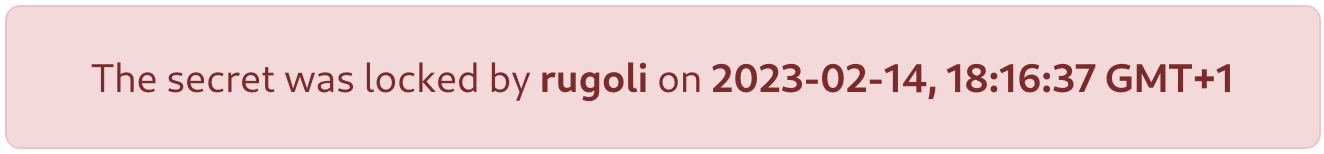
\includegraphics[width=0.8\linewidth]{img/unlock_warning.png}
    \captionof{figure}{Aviso del estado bloqueado de un secreto}
\end{center}


\subsubsection*{Borrar secreto}
{
\begin{minipage}{0.1\linewidth}
    
\includegraphics[width=\linewidth]{img/delete.png}
\end{minipage}
\hspace{0.5cm}
\begin{minipage}{0.9\linewidth}
    Un administrador, o usuario que tenga permisos para ello, podrá borrar un secreto con todas las consecuencias que ello conlleva: perder los datos, el histórico, no poder recuperarlo...
\end{minipage}
}

Debido a que es una acción que no se va a poder deshacer, se requerirá que el usuario realice una confirmación antes de que el secreto sea borrado.
\vspace{-8pt}
\begin{center}
    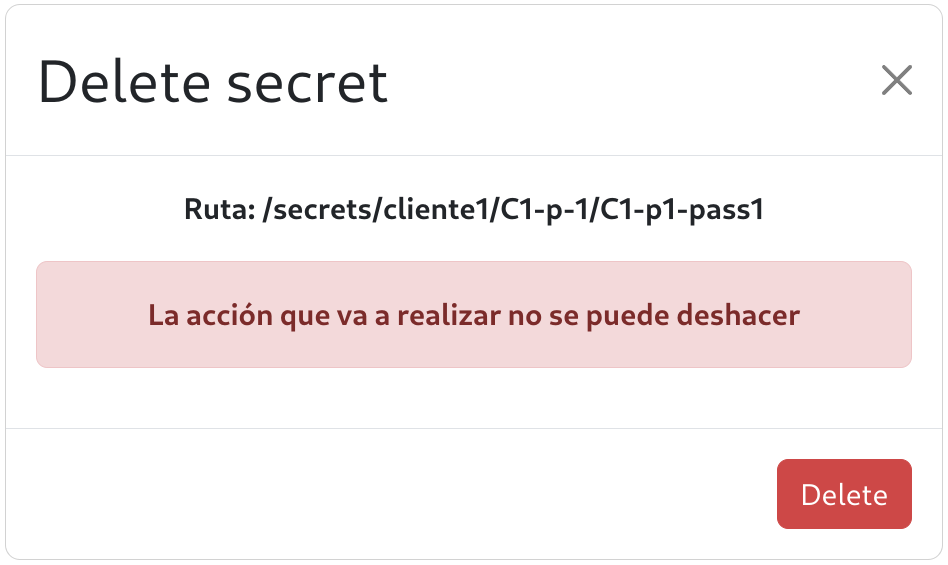
\includegraphics[width=0.6\linewidth]{img/delete_warning.png}
    \captionof{figure}{Confirmación al borrar un secreto}
\end{center}

Una vez el usuario haga \textit{click} en el botón de confirmación, el secreto se borrará y la aplicación redirigirá al usuario al directorio superior de donde se encontraba el secreto borrado.

\subsection{Editar un secreto}

Dado que esta acción es la más importante de la aplicación, se va a profundizar a continuación en las características del sistema de edición de secretos.

Tal como se ha visto en el apartado anterior, para editar un secreto existe un botón dedicado a tal acción. Al hacer \textit{click} sobre él, los botones de acción se ocultan y aparece el editor con los datos del secreto:

\begin{center}
    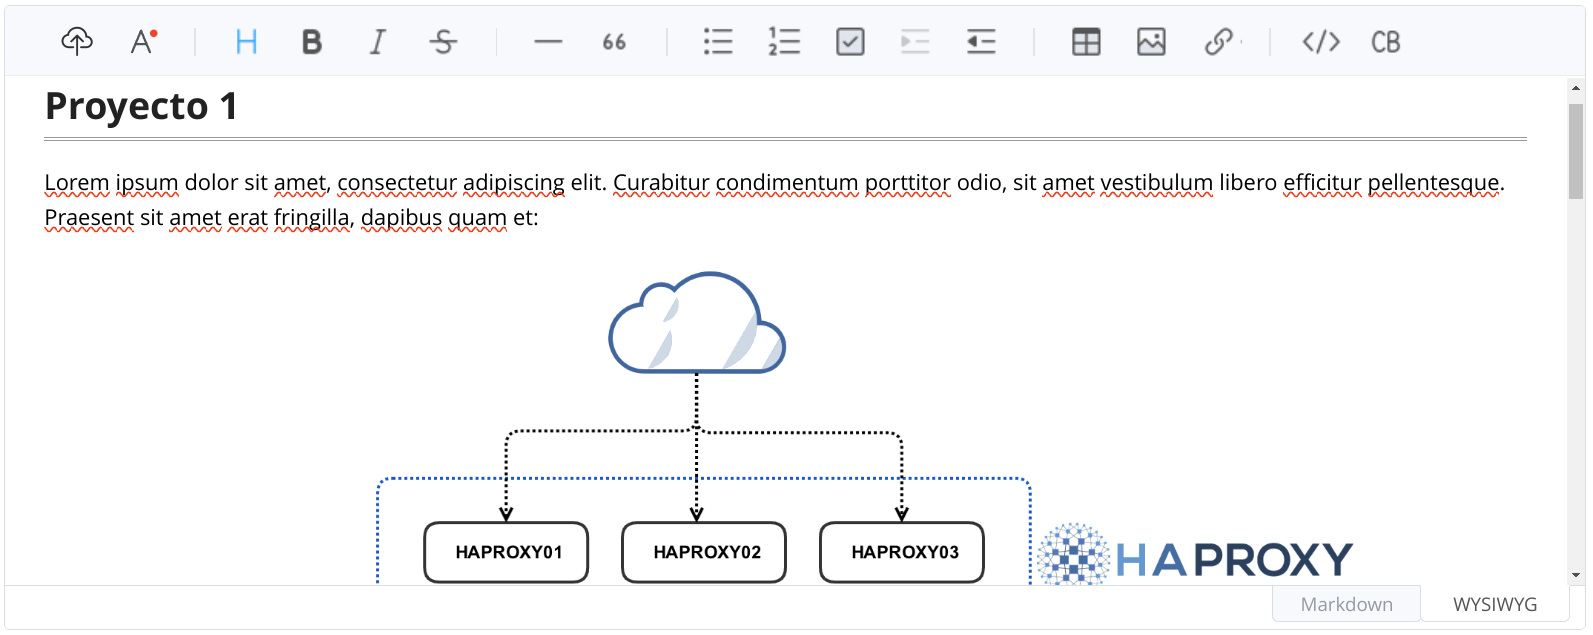
\includegraphics[width=\linewidth]{img/editor.png}
    \captionof{figure}{Editor \textit{WYSIWYG}}
\end{center}

El editor elegido es \href{https://github.com/nhn/tui.editor}{Tui.editor} ya que es un proyecto con \href{https://es.wikipedia.org/wiki/Licencia_MIT}{licencia MIT}, creado en el lenguaje \href{https://es.wikipedia.org/wiki/TypeScript}{Typescript} y que cumple con los requisitos para el proyecto.

Entre las características que tiene el editor, se pueden destacar:

\begin{itemize}
    \item Interfaz \textbf{WYSIWYG} (\textit{what you see is what you get}) completo que permite editar y guardar el documento generado en formato \href{https://es.wikipedia.org/wiki/Markdown}{Markdown}.
    \item Permite añadir imágenes arrastrándolas sobre el interfaz.
    \item Se puede expandir las funcionalidades a través de \textit{\textbf{plugins}}. Para este proyecto se están utilizando dos:
    \begin{itemize}
        \item Posibilidad de añadir \href{https://github.com/nhn/tui.editor/tree/master/plugins/color-syntax}{color al texto}, expandiendo las posibilidades de Markdown, ya que por defecto este sistema no lo permite.
        \item Mejoras en el \href{https://github.com/nhn/tui.editor/tree/master/plugins/color-syntax}{resaltado de sintaxis} a la hora de añadir bloques de código fuente o de configuración.

        Esto resulta es muy útil cuando se necesita guardar en la documentación configuración de algún tipo o fragmentos de código fuente. El plugin hace uso de \href{https://prismjs.com/}{PrismJS} que soporta 297 lenguajes.
        \begin{center}
            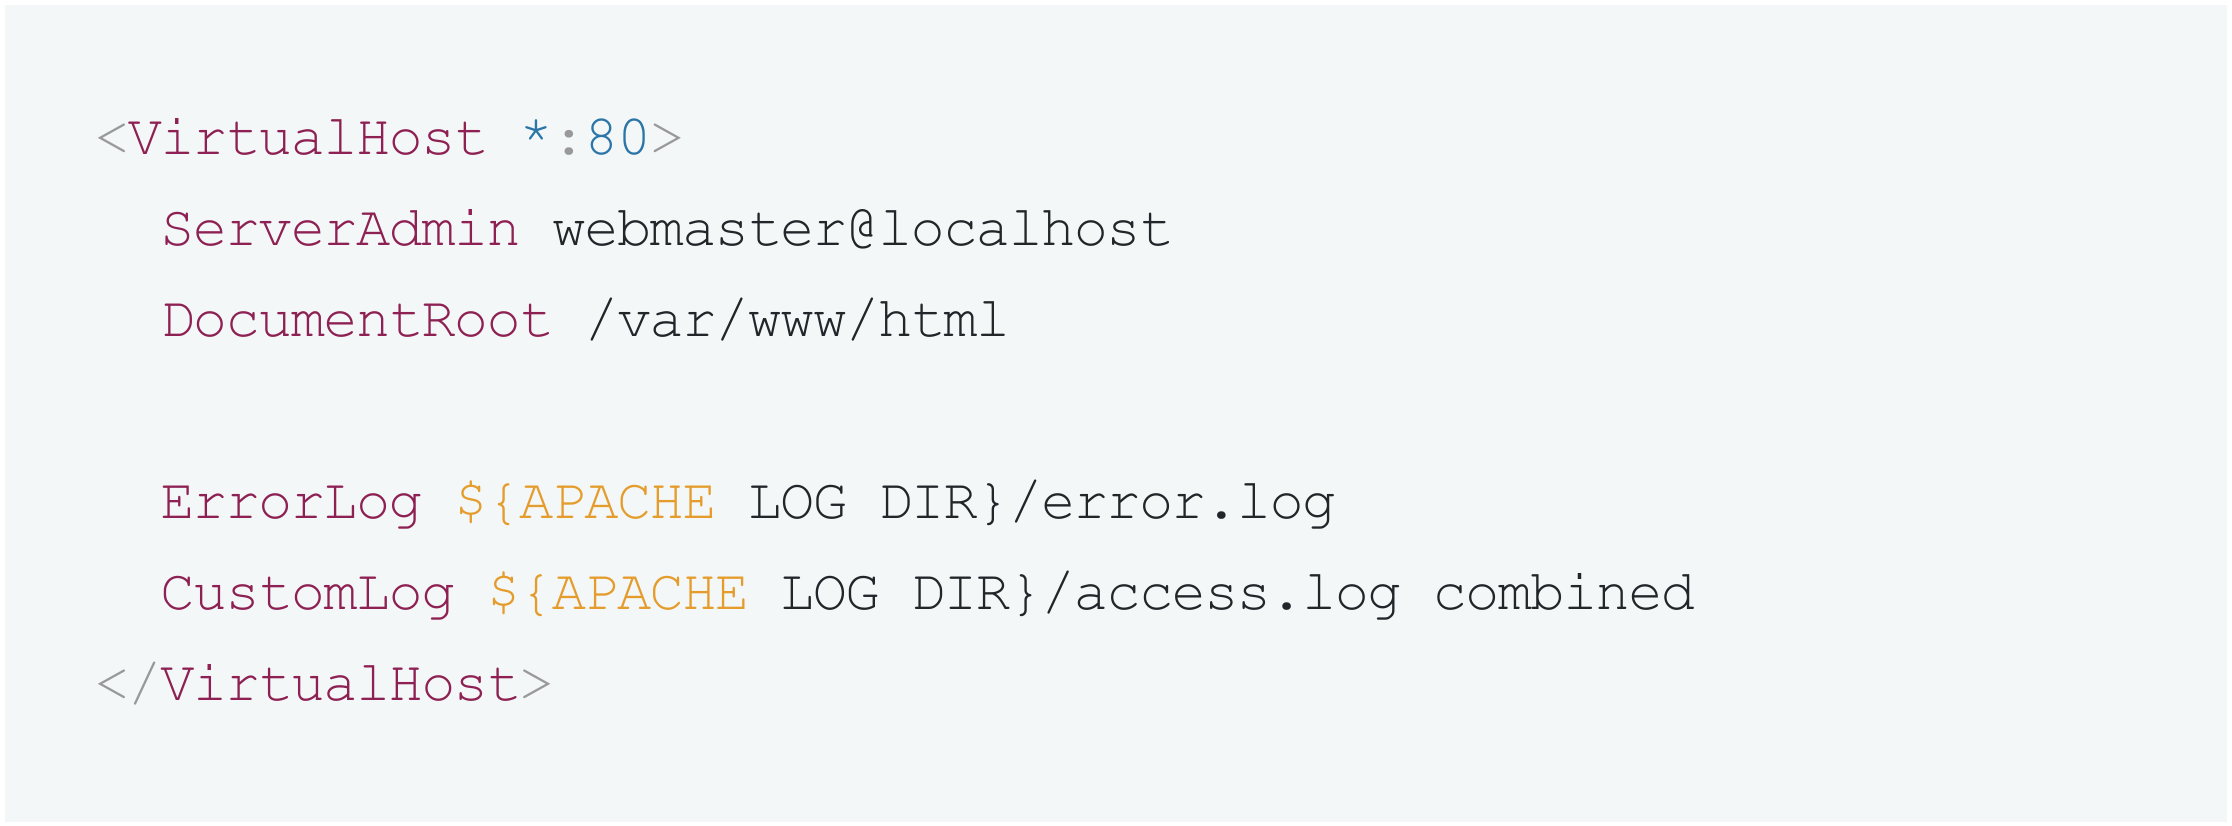
\includegraphics[frame,width=0.7\linewidth]{img/editor_example.png}
            \captionof{figure}{Ejemplo de resaltado de sintaxis}
        \end{center}
    \end{itemize}

    \item Posibilidad de añadir iconos propios a la barra de herramientas del editor. Esta característica ha sido clave ya que era necesario poder crear al menos un botón para guardar y cerrar el secreto.

    El icono añadido tiene el siguiente aspecto 
\includegraphics[width=0.8cm]{img/save_exit.png}. Al hacer \textit{click} sobre él, el secreto será guardado, el editor se cerrará y la aplicación nos redirigirá para que visualicemos el nuevo aspecto del secreto recién editado.
\end{itemize}

\subsection{Navegación por los secretos}

A la hora de navegar por las contraseñas y documentación se ha hecho uso de un sistema jerárquico que simula las carpetas de un explorador de archivos de cualquier sistema operativo actual.

Los usuarios están acostumbrados a hacer uso de cualquier tipo de ficheros y a ordenarlos en sus sistemas de almacenamiento, creando una jerarquía decidida previamente.

Dado que la aplicación se ha creado teniendo en cuenta las exigencias de una empresa para lidiar con contraseñas y documentación, se creía conveniente simular este sistema.

Para ello, se han creado 3 sistemas diferenciados en el interfaz, que funcionan en sincronía. Esto quiere decir, que al utilizar cualquier de ellos, hará que se actualice el resto.

\subsubsection*{Vista de árbol}
Es una visualización jerárquica de la información, que se ha situado en el lado izquierdo del interfaz. Este apartado visual siempre será visible en una pantalla de grandes dimensiones, como las de un ordenador de sobremesa.

Si por el contrario, la aplicación se está visualizando a través de un teléfono móvil, el árbol permanecerá oculto, aunque se podrá desplegar a través del botón de la parte superior derecha.

{
\begin{minipage}{0.3\linewidth}
    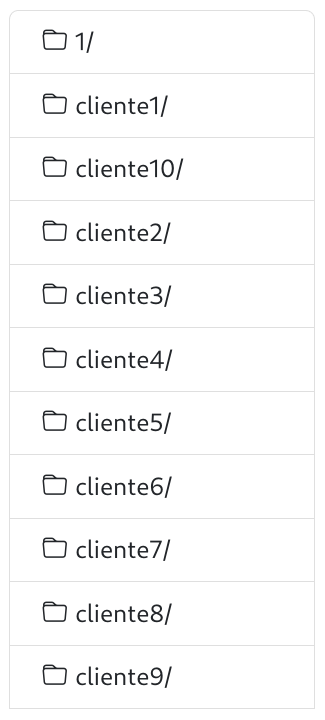
\includegraphics[width=0.9\linewidth]{img/tree1.png}
\end{minipage}
\hfill
\begin{minipage}{0.3\linewidth}
    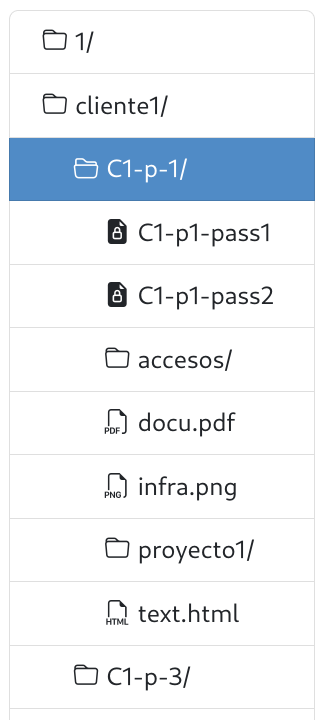
\includegraphics[width=0.9\linewidth]{img/tree2.png}
\end{minipage}
\hfill
\begin{minipage}{0.3\linewidth}
    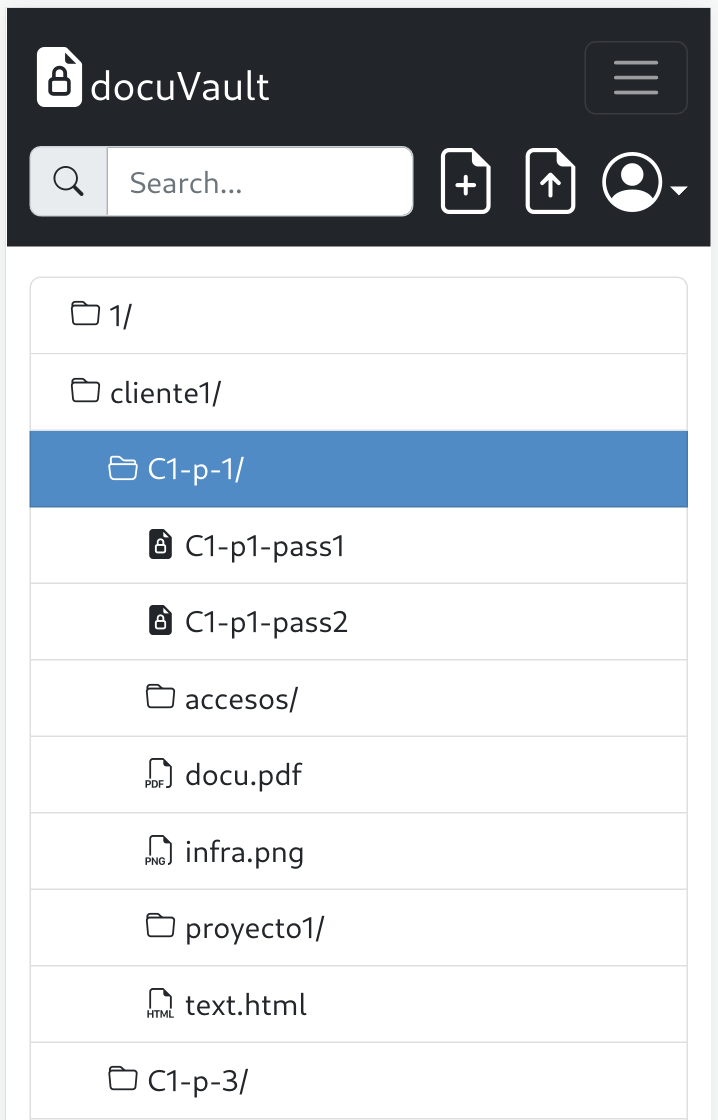
\includegraphics[width=\linewidth]{img/tree3.png}
\end{minipage}
\captionof{figure}{Detalles de la “vista de árbol” en modo normal y \textit{responsive}}
}

En la vista de árbol se pueden diferenciar:
\vspace{-10pt}
\begin{itemize}
    \item \textbf{Ramas}: Son los nodos que a su vez contiene otros nodos. En un explorador de ficheros serían los directorios.
    \item \textbf{”Hojas”}: Lo que en un explorador de archivos serían los ficheros.
\end{itemize}

Tal como se puede ver en las imágenes, al seleccionar cualquiera de los nodos, se resaltará la opción elegida con un color azul y se mostrará su contenido en caso de ser una rama.

\subsubsection*{Explorador de ficheros}

Es el método más habitual a día de hoy para navegar por un sistema de ficheros en los sistemas operativos modernos.

\begin{center}
    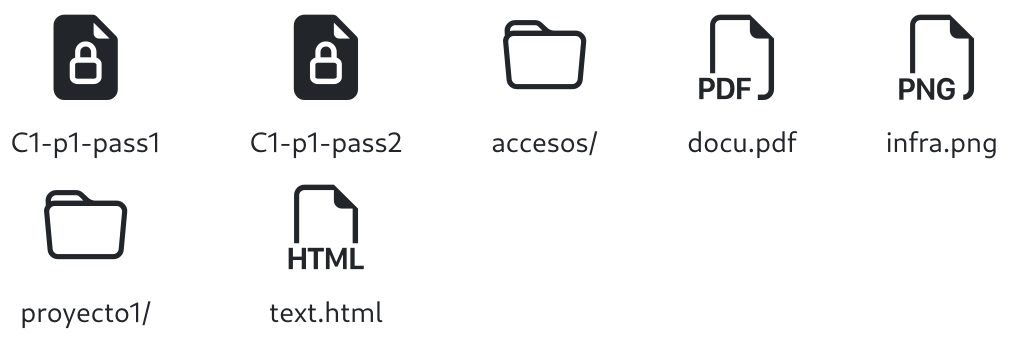
\includegraphics[width=0.9\linewidth]{img/browser.png}
    \captionof{figure}{Detalle del explorador de ficheros}
\end{center}

Para identificar el tipo de ficheros que se están visualizando se han identificado mediante distintos iconos. Los iconos utilizados son:

{
\begin{minipage}{0.1\linewidth}
    
\includegraphics[width=\linewidth]{img/folder.png}
\end{minipage}
\hspace{0.5cm}
\begin{minipage}{0.9\linewidth}
    Es un directorio, y al igual que sucede en un sistema de ficheros, puede contener a su vez otros ficheros y/o directorios.

    Al hacer \textit{click} sobre él, se visualizará su contenido. Esto afectará a la vista de árbol, que se actualizará para mostrar el directorio desplegado.
\end{minipage}
}


{
    \begin{minipage}{0.1\linewidth}
        
\includegraphics[width=\linewidth]{img/secret.png}
    \end{minipage}
    \hspace{0.5cm}
    \begin{minipage}{0.9\linewidth}
        Es un secreto creado y editado a través de la aplicación. Este icono nos identifica que al hacer \textit{click} visualizaremos su contenido, y posteriormente podremos realizar otras acciones como editarlo, imprimirlo, borrarlo...
    \end{minipage}
}


{
    \begin{minipage}{0.1\linewidth}
        
\includegraphics[width=\linewidth]{img/file.png}
    \end{minipage}
    \hspace{0.5cm}
    \begin{minipage}{0.9\linewidth}
        Existen distintas representaciones de iconos para identificar a ficheros que se han subido a la aplicación para ser cifrados y almacenados en ella.

        Dependiendo del tipo de fichero (identificado mediante la extensión) mostrará el tipo de fichero que es junto al icono. Existen iconos para las extensiones más habituales.
    \end{minipage}
}

Tal como se ha venido explicando hasta ahora, al simular algo que el usuario ya conoce se va a conseguir que el usuario utilice la aplicación para navegar y guardar la información, consiguiendo que la seguridad de la empresa mejore.


\subsubsection*{Navegación “miga de pan”}

La “miga de pan” (en inglés \textit{\textbf{breadcrumb}}) es una técnica de navegación que se utiliza en distintos tipos de interfaces gráficas de usuario para mostrar el camino recorrido.

Dependiendo de si estamos navegando en un directorio o si estamos en un fichero, al final aparecerá un símbolo “/” o no.

\begin{center}
    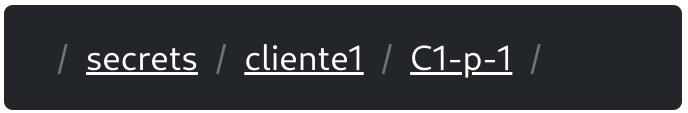
\includegraphics[width=0.6\linewidth]{img/breadcrumb1.png}
\end{center}
\begin{center}
    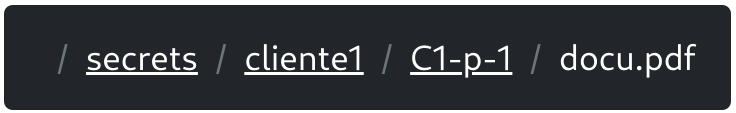
\includegraphics[width=0.6\linewidth]{img/breadcrumb2.png}
    \captionof{figure}{Detalle de la navegación con “miga de pan”}
\end{center}

Para poder volver sobre nuestros pasos, o para ir hacia arriba en la jerarquía, cada apartado de la “miga de pan” es un enlace, por lo que al hacer \textit{click} sobre cualquiera de ellos nos llevará a su correspondiente directorio.


\subsection{Subir un fichero al sistema}

Dado que la creación y edición de secretos puede resultar limitante, la aplicación permite la posibilidad de subir un fichero para que sea guardado y securizado.


{
    \begin{minipage}{0.1\linewidth}
        
\includegraphics[width=\linewidth]{img/upload.png}
    \end{minipage}
    \hspace{0.5cm}
    \begin{minipage}{0.9\linewidth}
        En la cabecera de la aplicación existe un icono que nos va a permitir subir a la aplicación un fichero de cualquier tipo. Al hacer \textit{click} sobre el icono, nos aparecerá un \textit{modal} para preguntarnos por la ruta donde queremos guardar el fichero y para que elijamos el fichero de nuestro sistema.
    \end{minipage}
}

\begin{center}
    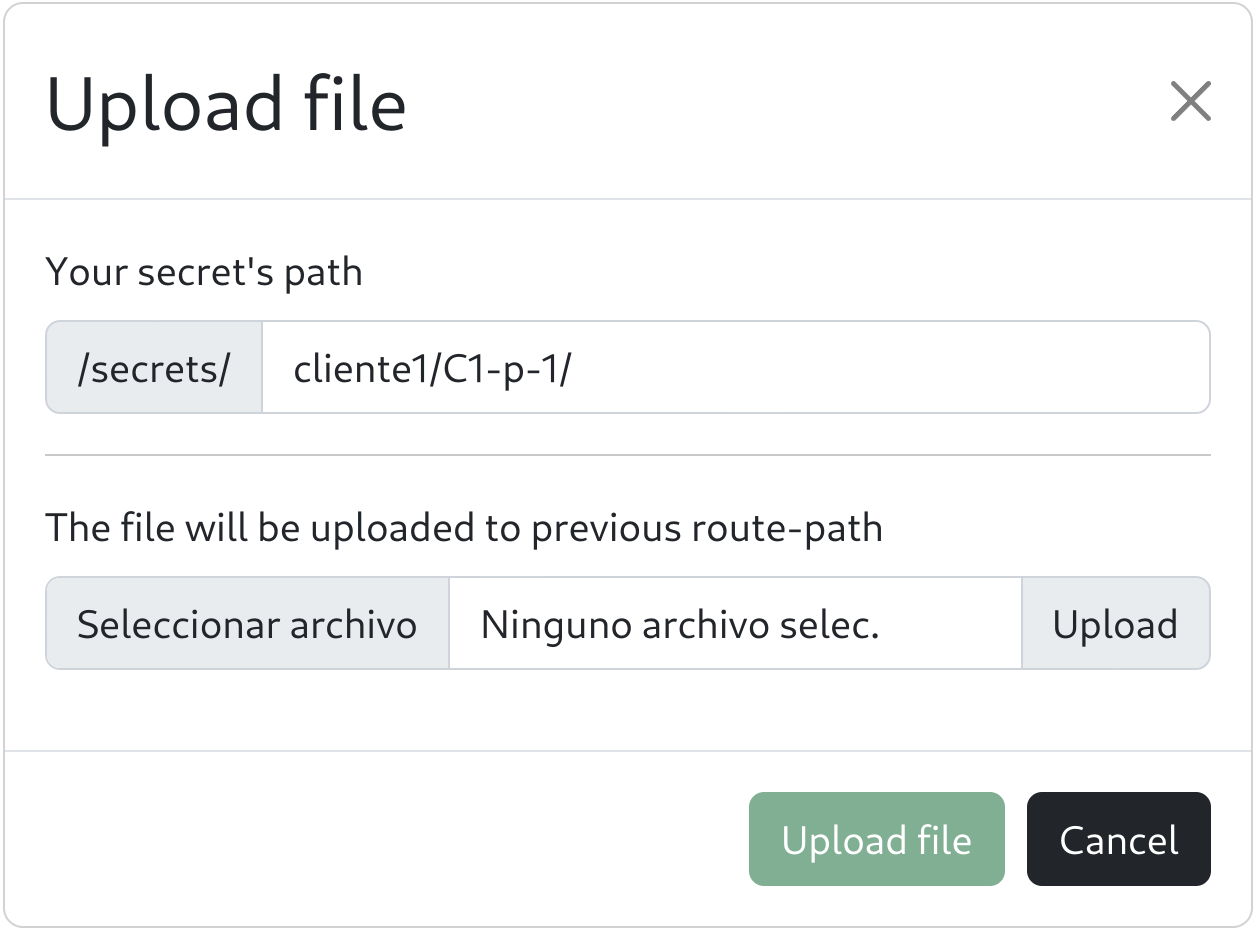
\includegraphics[width=0.7\linewidth]{img/upload_modal.png}
    \captionof{figure}{\textit{Modal} para subir un fichero}
\end{center}

Al igual que sucedía con la ventana para crear un secreto, este \textit{modal} también cuenta con un sistema de validación que no activará el botón hasta que no se elija del sistema un fichero o una ruta correcta.

Una vez la aplicación ha guardado el fichero de forma segura se nos redirigirá a la ruta donde se ha guardado. Para poder visualizar el fichero sin tener que descargarlo, el sistema detecta (a través del “\href{https://en.wikipedia.org/wiki/Media_type}{MIME Type}”) si es un fichero que se puede mostrar, y de esta manera lo visualizará.

Los ficheros que automáticamente se muestran son:

\begin{itemize}
    \item Ficheros \textbf{PDF}: El fichero se abrirá a través del lector de documentos del navegador, lo que posibilita su visualización o descarga.
    \item Ficheros de tipo \textbf{imagen}: Si el “MIME Type” es de tipo “\textbf{data:image}”, la aplicación creará un elemento en el HTML para poder visualizarlo.
\end{itemize}

\begin{center}
    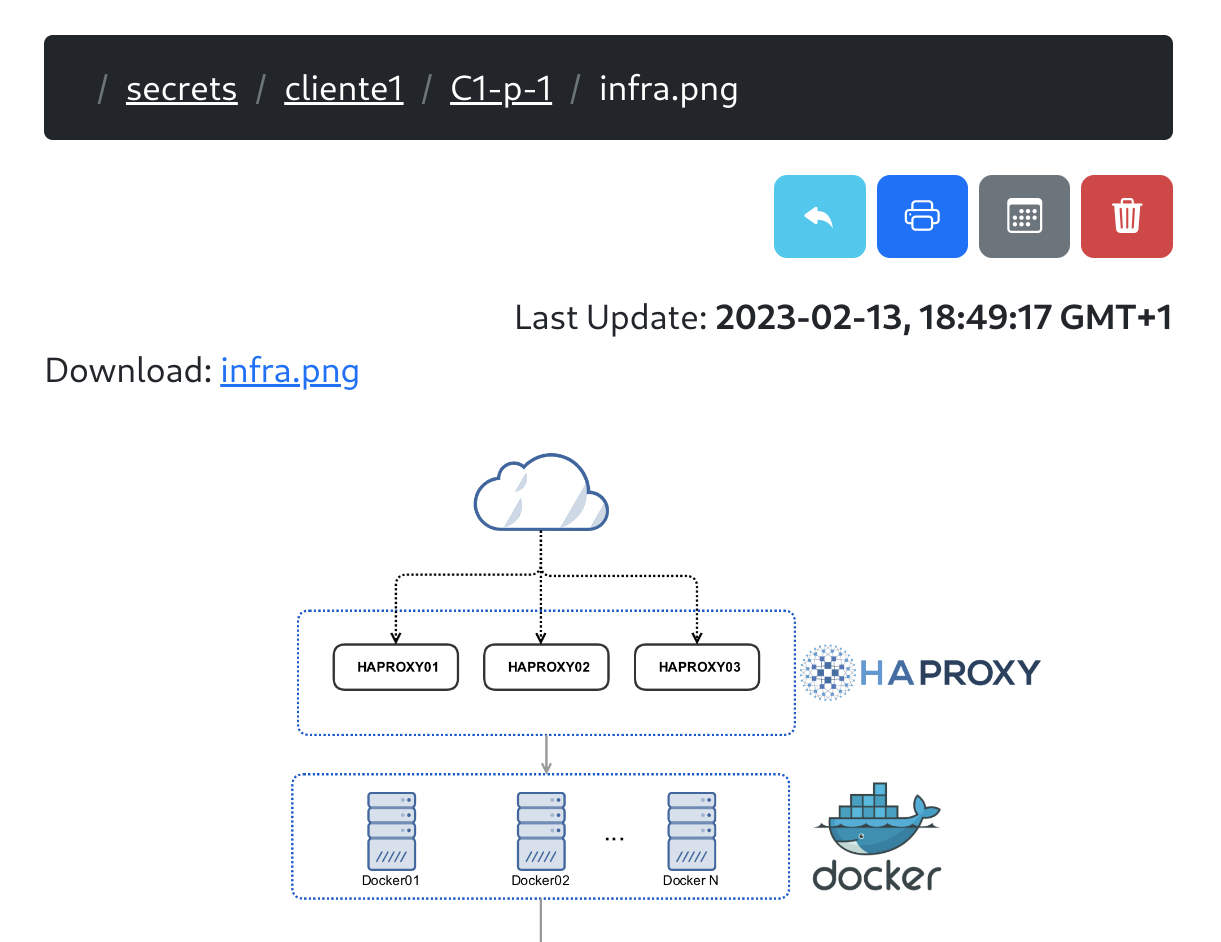
\includegraphics[frame,width=0.7\linewidth]{img/upload_download.png}
    \captionof{figure}{Visualización de un fichero subido a la aplicación}
\end{center}

Aparte, y tal como se puede ver en la imagen superior, aparecerá un enlace para poder descargar el fichero subido, lo que permitirá recuperar el archivo sin cifrar.


\section{Vault como \textit{backend} de información}

Ya se ha comentado previamente cómo Vault es un proyecto para asegurar, almacenar y controlar el acceso a secretos. La idea de la aplicación realizada ha sido explotar esas funcionalidades y llevarlas un paso más lejos para adaptarlas a un entorno de documentación.

La comunicación con Vault se realiza a través de su \href{https://developer.hashicorp.com/vault/api-docs}{API}, por lo que el servicio debe de estar funcionando y en parte configurado para que la aplicación funcione sobre él.

Tal como se lleva repitiendo a lo largo del documento, la aplicación creada trata de buscar ser una herramienta que pueda servir en una empresa como sistema centralizado para la securización de contraseñas y documentación. Es por eso que debe de realizarse una configuración previa para que la aplicación funcione.

\subsection{Configuración inicial de Vault}

Dado que Vault va a ser el sistema que se va a encargar del almacenamiento de los secretos es vital que su instalación y configuración inicial sea correcta.

Los pasos que deben realizarse están explicados en su \href{https://developer.hashicorp.com/vault/tutorials/getting-started/getting-started-deploy}{documentación oficial}, pero a continuación se van a simplificar rápidamente:

\begin{itemize}
    \item Crear un \textbf{servicio de inicio automático} para que en caso de que el servidor se reinicie, el servicio arranque de manera automática. En sistemas GNU/Linux se puede hacer a través de Systemd.
    \item \textbf{Configurar Vault}: Teniendo distintos puntos a tener en cuenta que se van a detallar en los apartados siguientes.
    \item \textbf{Inicializar Vault}: Al inicializar Vault se generarán el \textit{\textbf{token inicial de root}} que es el que permite la administración completa del servicio. Es fundamental guardarlo a buen recaudo.

    También se generan las \textbf{claves de \textit{unseal}} para abrir el acceso a los secretos. Cuando Vault arranca no es posible acceder a los secretos hasta que no se ha realizado el proceso de \textit{unseal}.
\end{itemize}

A continuación se van a detallar las decisiones que una empresa puede tomar a la hora de configurar Vault para que se adapte mejor a sus necesidades.

\subsection{Sistema \textit{backend} de autenticación}

En una empresa lo habitual es hacer uso de un sistema centralizado de autenticación, para que todos los usuarios se generen en la misma plataforma.

Hoy en día, los métodos más habituales suelen ser:
\begin{itemize}
    \item \textbf{Directorio Activo de Windows Server}: en empresas donde se haga uso de Windows como sistemas de escritorio, es habitual que el sistema de autenciación esté centralizado y junto con él se hagan usos de sistemas de seguridad como GPOs, carpetas compartidas, ...
    \item \textbf{LDAP}: Un sistema más estandarizado es el de LDAP, que también se puede integrar con otro tipo de aplicaciones.

    \item \textbf{Gestión de usuarios local}: En caso de que no se quiera integrar Vault con sistemas internos de la empresa, Vault cuenta con su propia gestión de autenticación para usuarios.
\end{itemize}

Cada empresa tendrá que decidir cuál es el mejor método que se adapta a ella, y adaptar la aplicación a ella, tarea que resulta sencilla.


\subsection{\textit{Key/Value} como motor de secretos}
Para la interacción con los secretos se ha decidido hacer uso del sistema “\href{https://developer.hashicorp.com/vault/api-docs/secret/kv/kv-v2}{KVv2}” que tiene integrado Vault. Este sistema nos ofrece:

\begin{itemize}
    \item Sistema de interacción \textbf{clave-valor}, habitual en bases de datos no relacionales.
    \item Interactuar con los secretos de manera sencilla a través de la API.
    \item Modificar los \textit{metadata} para poder guardar un histórico de lo sucedido.
    \item Tener un sistema de versiones por cada secreto.
\end{itemize}

Esta es la característica más importante utilizada por parte de la aplicación a la hora de interactuar con Vault.


\subsection{\textit{Backend} de almacenamiento}

Este es otro punto que la empresa debe tener en cuenta a la hora de configurar Vault, ya que de ello dependerá cómo se almacenen los secretos en el servidor final (aunque siempre se realiza de manera cifrada).

Existen distintos \href{https://developer.hashicorp.com/vault/docs/configuration/storage}{\textit{backends} de almacenamiento} y dependiendo de las necesidades se deberá optar por uno u otro.

\begin{itemize}
    \item \textbf{\textit{Filesystem}}: Es el método más sencillo de implementar, ya que Vault almacena los secretos en formato de ficheros en el servidor.
    \item \textbf{Bases de datos}: Dependiendo del sistema de base de datos utilizado podríamos hacer uso de su sistema en alta disponibilidad para tener un sistema escalable (como se puede realizar con MySQL).
    \item \textbf{S3}: Quizá interese almacenar los secretos en un \textit{bucket} S3 de Amazon, y de esta manera no depender de almacenamiento local.
\end{itemize}

Estos son sólo unos ejemplos de los distintos sistemas de almacenamiento que se pueden utilizar. Habría que tomar la decisión de cuál elegir y realizar la configuración en Vault. La opción elegida será transparente para la aplicación que se ha creado.


\section{Angular: Aspectos destacables de la programación}

Tras explicar cómo funciona la aplicación desde el punto de vista del usuario, se va a profundizar en algunos aspectos técnicos realizados durante la programación.

Tal como se ha dicho, la aplicación está programada utilizando el \textit{framework} \href{https://angular.io/}{Angular} y por tanto se ha hecho uso del lenguaje \href{https://www.typescriptlang.org/}{Typescript}.

A continuación se van a detallar algunos aspectos importantes y algunas características utilizadas durante la programación de la aplicación.


\subsection{Vistas en componentes separados}

Durante la creación del interfaz gráfico se ha dividido en distintos componentes para de esta manera diferenciar el código de la vista para cada uno de ellos.

\begin{center}
    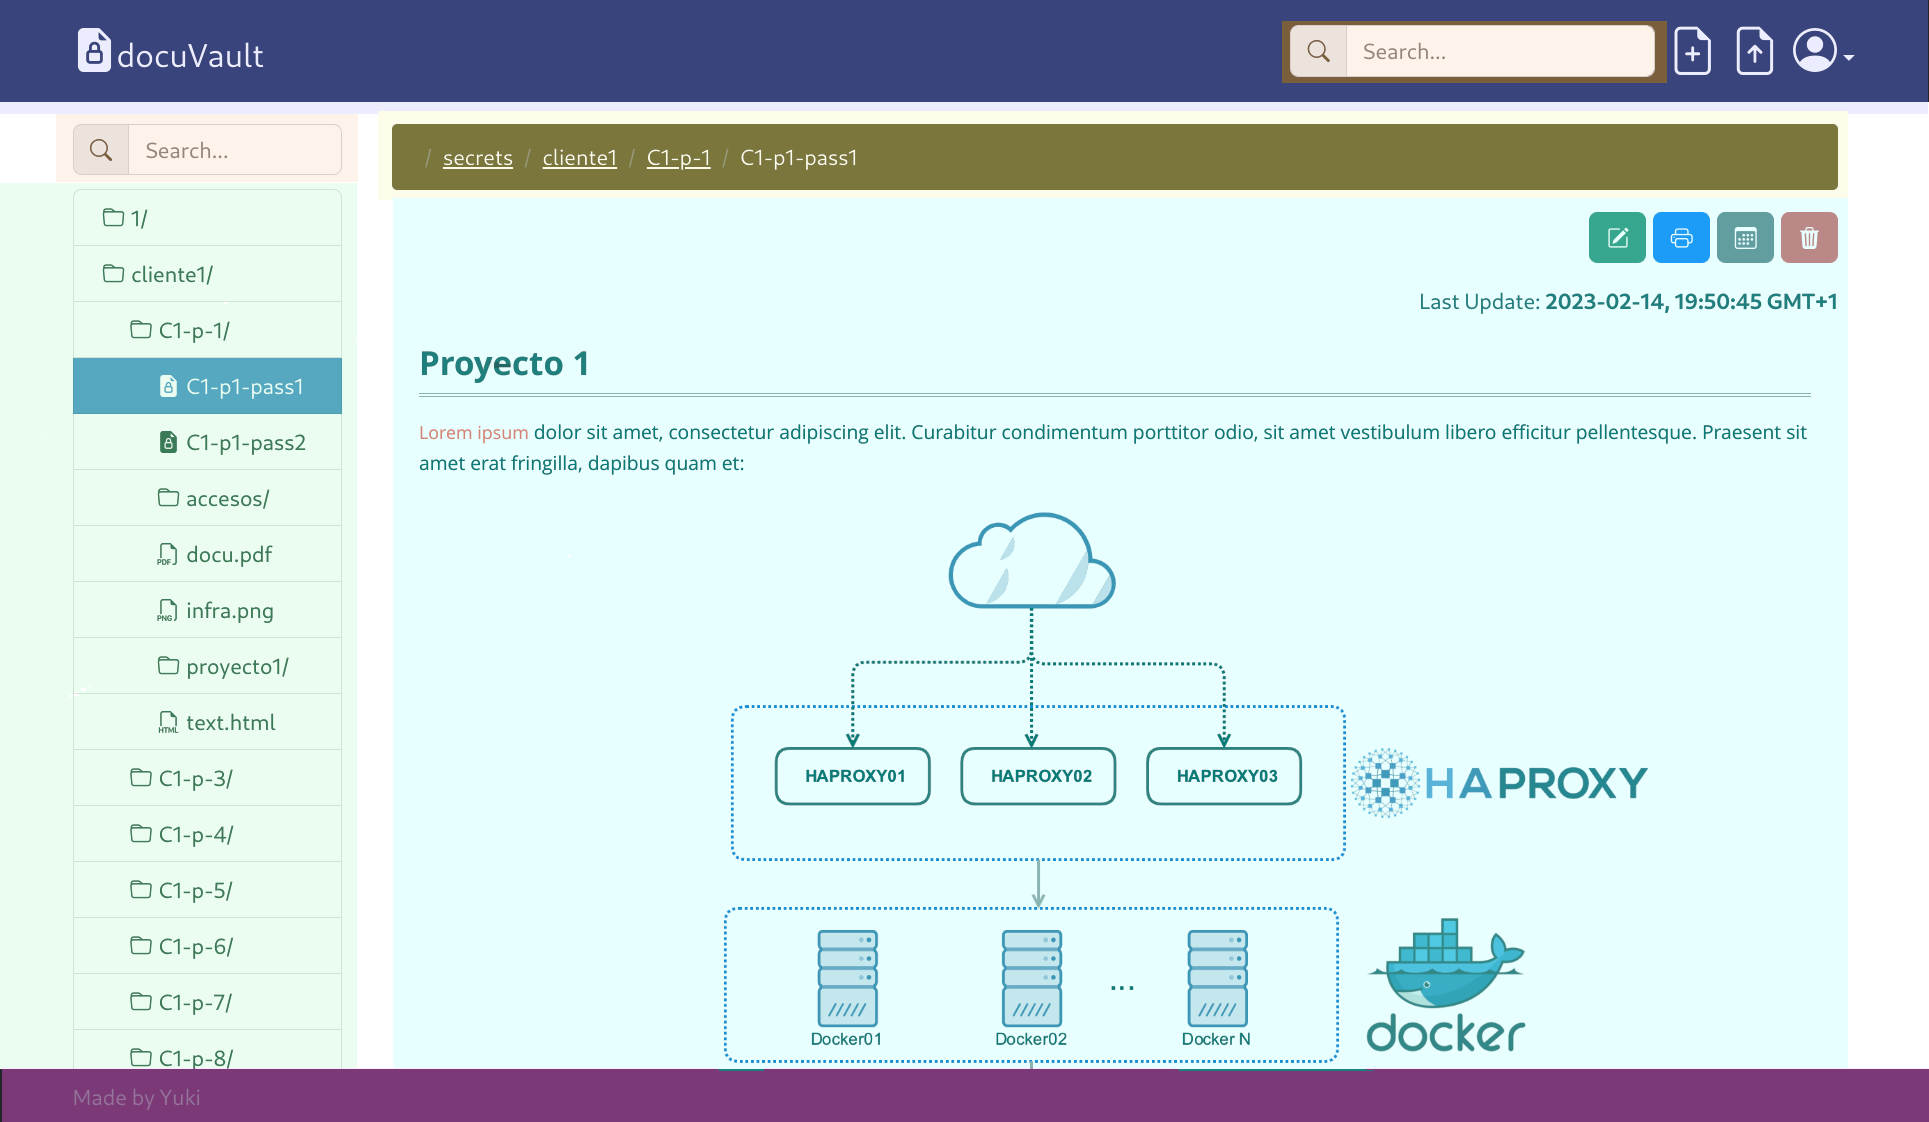
\includegraphics[frame,width=\linewidth]{img/interfaz2-colored.png}
    \captionof{figure}{Interfaz principal con los componentes coloreados}
\end{center}

En la imagen se han coloreado los distintos componentes que existen a la hora de visualizar un secreto:

\begin{itemize}
    \item \textbf{Cabecera}: La cabecera de la aplicación una vez el usuario se ha logueado.
    \item \textbf{Cajón de búsqueda}: Este componente se reutiliza en dos partes del interfaz: en la cabecera y encima de la vista de árbol de secretos.
    \item \textbf{Vista de árbol}: Este componente se oculta cuando el interfaz está siendo visualizado en una pantalla pequeña.
    \item \textbf{Breadcrumb} o “miga de pan”: Este es el componente que nos visualiza la ruta en la que nos encontramos.
    \item \textbf{Vista del secreto}: Esta es la vista principal cuando se está visualizando el secreto. En caso de que se esté editando el secreto, la vista mostrará el editor.
    \item \textbf{Pie de página}: El pie de página de la aplicación.
\end{itemize}

Aparte de los componentes explicados previamente, existen otro dos:

\begin{itemize}
    \item \textbf{Login}: Es el encargado de mostrar el \textit{modal} del \textit{login} cuando no se está logueado en la aplicación.
    \item \textbf{Explorador de ficheros}: Es el componente que visualiza los secretos como si fuese un explorador de ficheros.
\end{itemize}

\begin{center}
    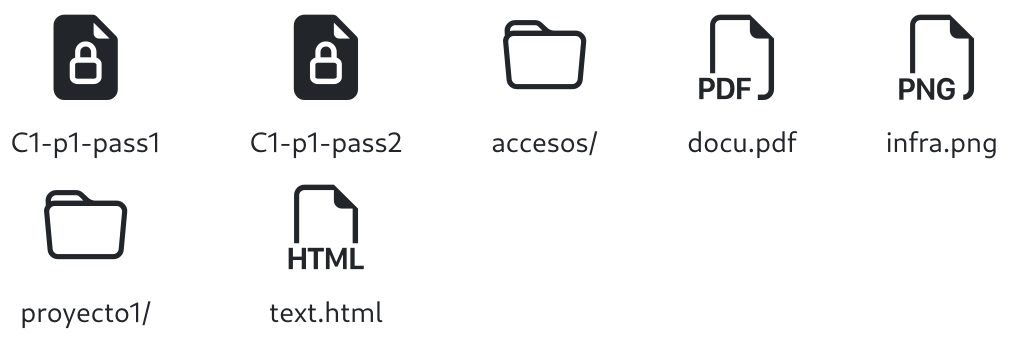
\includegraphics[width=0.9\linewidth]{img/browser.png}
    \captionof{figure}{Detalle del explorador de ficheros}
\end{center}


Varios de estos componentes están integrados en la vista principal a la hora de iniciar la aplicación, en el fichero \configfile{app.component.html}.

\begin{mycode}{Fichero app.component.html}{html}{}
<app-header></app-header>
<div class="container pt-3 mb-5">
    <div class="row">
        <div id="tree_navbar" class="col-md-3 col-lg-2 d-md-block sidebar
         collapse d-print-none">
            <app-tree></app-tree>
        </div>
        <main class="col-md-9 ms-sm-auto col-lg-10 px-md-4">
            <app-breadcrumb></app-breadcrumb>
            <app-browser></app-browser>
            <router-outlet></router-outlet>
        </main>
    </div>
</div>
<app-footer></app-footer>
\end{mycode}


Dado que los componentes idealmente sólo deben centrarse en la experiencia de usuario, se detallará cómo se ha realizado el paso de información entre ellos.



\subsection{\textit{Services} e inyección de dependencias}

Para la obtención de datos de los secretos a través del \textit{backend} Vault utilizando su \href{https://developer.hashicorp.com/vault/api-docs}{API}, y para la sincronización y envío de información entre los distintos componentes de la vista se ha creado un servicio en Angular, cuya dependencia se ha inyectado al inicio de la aplicación.

El servicio ha facilitado que distintos componentes que van a visualizar parte de la misma información (como la vista de árbol y el explorador de ficheros), o que dependen unos de otros, van a estar en sincronía a través del servicio.


\subsection{Programación asíncrona con \textit{promises}}

Dado que gran parte de la aplicación se basa en comunicarse con la API de Vault, ha sido necesario hacer uso en todo momento de la programación asíncrona al realizar las peticiones.

El ejemplo más claro es la generación del árbol de secretos. Para ello se ha hecho un algoritmo recursivo de petición a la API de los secretos, que cuando comprobaba que existía una jerarquía de directorios, debía entrar al directorio y recorrerlo recursivamente.

Al finalizar, las \textit{promises} hay que resolverlas para generar la estructura jerárquica que luego se convierte en la vista de árbol.

\begin{mycode}{Resolviendo \textit{promises} de la función recursiva}{typescript}{}
// Cogemos las promesas y las resolvemos
Promise.all(promises).then(data => {
    data.forEach((value:any) => {
        if (value != null){
            var x = nodes.map(function(e:any){
                return e.href
            }).indexOf(value[0].path)
            // cada nodo pertenece a un padre
            nodes[x].nodes = value
        }
    });
    resolve(nodes)
});
\end{mycode}

Angular, y ciertas peticiones que podemos realizar a través de la red, hace uso de \textit{observables}, que funcionan de manera similar a las \textit{promises}.

\subsection{Envío de mensajes con \textit{observables}}

Para la comunicación entre componentes, y también para consolidar la información a través de la API de Vault con la vista, se ha hecho uso de distintas variables de tipo \textbf{\textit{Observable}}.

Este tipo de variables hacen uso del patrón conocido como “\textit{\textbf{publish-subscribe}}”, en el que desde un \textit{subject} se mantiene una lista de \textit{observers} que dependen de él.

De esta manera, cuando se envía un mensaje, los observadores reciben esa información de manera asíncrona para posteriormente utilizarla en la vista en la que está escuchando.

En el siguiente ejemplo se va a detallar parte de la información que se puede encontrar en el \textit{Service} creado llamado \textbf{VaultServices}, en el que se inicializa una variable “secret\_history” que contendrá información de las distintas versiones de un secreto.

A través de la función “get\_secret\_history()” se realizarán peticiones a la API de Vault (usando otra función propia), para posteriormente generar un \textit{array} de la información que posteriormente se enviará a los subscriptores que están a la espera.

\begin{mycode}{Creamos \textit{Observable} y mandamos información}{typescript}{{\small }}
export class VaultService {
    //...
    public secret_history = new Subject<object>()
    public secret_history$ = this.secret_history.asObservable()
    //...
    public get_secret_history(){
        this.get_path(this.actual_url,"metadata").subscribe((resp:any) => {
            let versions:any = []
            let versions_keys = Object.keys(resp.data.versions)
            for (let index = 0; index <= versions_keys.length-1; index++) {
                versions.push([versions_keys[index],
                  resp.data.versions[versions_keys[index]]])
            }
            //enviamos información
            this.secret_history.next(versions.reverse())
        })
    }
}
\end{mycode}

Continuando con el ejemplo, desde la vista en la que se visualiza a un secreto, se puede ver cómo se ha creado una suscripción a la variable detallada previamente, que al recibir información actualizará la variable local “versions”.

\begin{mycode}{Ejemplo de subscripción a un \textit{Observable}}{typescript}{}
export class SecretComponent implements OnInit {
    versions: any = null

    constructor(
        protected vault: VaultService,
    ) {
        //...
        this.vault.secret_history.subscribe(secret_history => {
            this.versions = secret_history
        })
    }
}
\end{mycode}

Esta variable, para terminar, es utilizada en la vista para generar una lista con las distintas versiones con las que cuenta el secreto:

% pongo “hybris” porque el formato html+ng2 me la lía
\begin{mycode}{Uso de la variable  en la vista}{hybris}{}
<ul *ngFor="let version of versions; index as i">
  <li><a routerLink="/v/{{version[0]}}{{this.vault.actual_url}}"
    (click)="modal.dismiss('Cross click')">
      <strong>v{{version[0]}}</strong>:
        {{version[1].created_time|date: "yyyy-MM-dd, HH:mm:ss z"}}
    </a>
  </li>
</ul>
\end{mycode}

Este tipo de secuencia “llamada a la API de Vault → envío de información al suscriptor/suscriptores → recibir información → actualizar vista” se repite de manera continuada a lo largo de toda la aplicación.


\chapter{Trabajo futuro}

Dada la naturaleza de la aplicación realizada, y las distintas posibilidades que puede aportar dentro de una empresa, se podría decir que el trabajo futuro a desarrollar es tan diverso como las necesidades de las empresas que lo puedan utilizar.

Actualmente la aplicación se considera que es funcional dentro de las tareas que puede realizar, y que por tanto se podría hacer uso de ella para un entorno en producción dentro de cualquier tipo de empresa.

Es cierto que las funcionalidades que tiene actualmente se pueden considerar básicas, pero eso facilita que la aplicación ya pueda ser utilizada. Teniendo en cuenta las metodologías ágiles de desarrollo utilizadas, es cuestión de escuchar la opinión de los usuarios para ir aportando valor y de estar manera ir ampliando las funcionalidades.

Con todo ello, dado que existen muchas funcionalidades que se han quedado sin realizar, y que podrían interesar a nivel general, a continuación de detallan un número de funcionalidades que podrían ir añadiéndose a la aplicación en futuros \textit{sprints}:

\begin{itemize}
    \item \textbf{Panel de control para administradores}: Como muchas aplicaciones, va a existir el rol de administrador, y que por tanto será el encargado de administrar no sólo la gestión del servicio, si no también la creación de usuarios como de dar permisos.

    Es por eso que sería interesante crear una ruta dentro de la aplicación a la que sólo los administradores puedan acceder y donde se podrían efectuar las siguientes tareas:

    \begin{itemize}
        \item \textbf{Gestión de usuarios}: Si no se hace uso de un sistema centralizado de usuarios (como \textit{Active Directory} o LDAP), es conveniente tener un lugar donde crear usuarios, borrarlos, cambiarles la contraseña...
        \item \textbf{Gestión de permisos}: Para crear las políticas de permisos de los usuarios.
        \item \textbf{Gestionar secretos bloqueados}: Tener un lugar donde desbloquear posibles secretos que se hayan quedado bloqueados.
        \item \textbf{Auditoría completa}: Vault cuenta con un sistema completo de auditoria, que es capaz de guardar logs por cada acción de usuario. Dada la importancia de este tipo de información, podría ser recomendable guardarlo en un sistema de base de datos no-relacional y poder acceder a dicha información en cualquier momento.
    \end{itemize}

    \item \textbf{Crear configuración para el usuario}: Crear un área de configuración para el usuario. En este apartado, algunas opciones que podría configurar son:

    \begin{itemize}
        \item Cambiar el aspecto visual de la aplicación. Ya sea a través de distintos temas o simplemente entre un tema claro y otro oscuro.
        \item Permitir forzar la actualización de la vista de árbol.
        \item Decidir si quiere tener la vista de árbol siempre visible.
    \end{itemize}

    \item \textbf{Auditoría propia para los secretos}: Crear un sistema propio más sencillo que el que tiene de serie Vault para conocer las modificaciones históricas de quién ha modificado el secreto.

    \item \textbf{Ver diferencias entre versiones}: Actualmente se pueden ver las distintas versiones de un secreto, pero pueder ser interesante seleccionar dos versiones y ver cuáles son las diferencias entre las dos versiones. Sería tener una herramienta similar a \commandbox{git diff}.

    \item \textbf{Creación de “timers”}: La idea sería que si un usuario no utiliza la aplicación en X minutos, se realice un deslogueo de la aplicación. De esta manera, se salvaguardan los datos ante posibles accesos a un equipo que no está siendo utilizando en un momento dado.

    \item \textbf{Mejoras en la visualización de secretos}: Mejorar y ampliar la visualización de los distintos tipos de ficheros que se pueden subir a la aplicación.

    Puede ser interesante permitir la visualización de documentos tipo word, libreoffice, excel,... haciendo uso de librerías externas.

    \item \textbf{Crear un índice en los secretos creados}: Dado que la aplicación permite crear documentos gracias al sistema Markdown, se entiende que estos documentos pueden contar con una jerarquía interna basada en encabezados.

    Sería interesante que antes de visualizar el secreto, \textit{parsearlo} para generar una “tabla de contenidos” (TOC o \textit{table of contents} en inglés), y de esta manera generar índices para poder llegar a la parte que interese del documento.

    \item \textbf{Generar e-mail para enviar un secreto}: Junto con la opción de imprimir el secreto, puede ser interesante la opción de crear un botón para generar automáticamente un e-mail para enviar el secreto.

    Como alternativa, y para no tener que enviar la información, se podría generar un token que dure un periodo de tiempo determinado, y que al generar el e-mail se mande dicho token. El usuario receptor deberá loguearse con dicho token para poder visualizar la información.
\end{itemize}

Tal como se puede observar, el número de nuevas funcionalidades con las que mejorar la aplicación puede resultar muy amplia, y tal como se ha dicho previamente, todo ello sin tener en cuenta la opinión de los usuarios finales.

Con todo ello, y teniendo en cuenta las posibilidades que este tipo de aplicación puede llevar a una empresa, resulta interesante pensar las posibles funcionalidades que podría llegar a tener en un futuro.



\vfill
\pagebreak
\chapter{Conclusiones}

La seguridad a la hora de almacenar datos importantes, y salvaguardar las contraseñas de accesos a servicios debe ser una prioridad a nivel personal, pero mucho más cuando hablamos a nivel empresarial. En este último caso puede llegar a haber consecuencias legales en caso de perder esa información (ya sea por borrado o por filtraciones por ataques de agentes externos).

A pesar de que ya existen herramientas dedicadas a guardar contraseñas, se ha demostrado que este tipo de aplicaciones comerciales no están exentas de fallos de seguridad, y que debido a la importancia de las mismas, suelen ser objetivos de ataque para la obtención de información sensible.

Aún existiendo aplicaciones de Software Libre para el mismo fin, en las que la comunidad se vuelca para que tales fallos de seguridad no existan, normalmente sólo están dedicadas a guardar contraseñas, sin posibilidad de crear documentación en la propia aplicación. Existe la posibilidad de modificar estas aplicaciones, gracias a las licencias libres que las componen, pero puede suponer un esfuerzo que puede no estar al alcance de muchos.


A lo largo de este trabajo final de máster se ha demostrado cómo crear una herramienta \textit{ad hoc} para guardar contraseñas, subir ficheros y donde se puede crear y editar documentación no es una tarea demasiado compleja y que puede ser llevado por cualquier empresa tecnológica que cuente con un desarrollador que tenga conocimientos de programación.

Las ventajas de crear una aplicación propia, y securizarla para limitar el acceso a la misma, trae consigo una serie de ventajas que un producto comercial es difícil que consiga. Podremos adaptar la aplicación a medida que la empresa vaya necesitando nuevas características, y por tanto no nos limitaremos a lo que un producto de terceros nos permita hacer.

Por último, y dado que para la creación de la aplicación nos hemos basado en herramientas con licencia de Software Libre, al dotar a nuestra aplicación del mismo tipo de licencia, estaremos permitiendo a la comunidad que incluyan mejoras de cualquier tipo. Esto no sólo es beneficioso para la propia comunidad, si no también para las empresas, que podrán añadir esas nuevas características a su propio desarrollo, mejorando así su propia aplicación interna.




\vfill

\pagebreak
\printbibliography[title={Referencias bibliográficas},heading=bibintoc]
\pagebreak

{
    \addcontentsline{toc}{chapter}{\listfigurename}
    % un poco de ñapa para quitar el color a los enlaces
    \hypersetup{linkcolor = black}
    \listoffigures
}

\end{document}
